\documentclass{eceasst}
% This is the source of the author documentation
% for the ECEASST document class.

% Required packages
% =================
\usepackage{subfig}

\usepackage{orcidlink}
\usepackage{accsupp}
\usepackage{todonotes}
\usepackage{lineno}


\usepackage{booktabs}
\usepackage{longtable}
\usepackage{array}

% Left-aligned columns with automatic line wrapping
\newcolumntype{P}[1]{%
  >{\raggedright\arraybackslash}p{#1}}


\linenumbers

\usepackage[ngerman,british]{babel}
\newenvironment{de}{\begin{otherlanguage}{ngerman}}{\end{otherlanguage}}
\newenvironment{en}{\begin{otherlanguage}{british}}{\end{otherlanguage}}

%Mathematical formula accessibility and machine-readability: if you add
\usepackage[accsupp]{axessibility}
\pdfcompresslevel=1
%in the article preamble, you can select an equation and copy-paste it to a text file to recover the TeX math


% PDF accessibility and PDF metadata
\newcommand{\authorRef}[1]{\texorpdfstring{\autref{{#1}}}{}}
\newcommand{\authorOrcid}[1]{\texorpdfstring{\thinspace\orcidlink{#1}\thinspace}{}}
\newcommand{\geprislink}[1]{\href{https://gepris.dfg.de/gepris/projekt/#1?language=en}{#1}}

\newcommand{\Eg}{E.\,g.}
\newcommand{\eg}{e.\,g.}
\newcommand{\ie}{i.\,e.}

\newcommand{\elabftw}{\href{https://www.elabftw.net/}{eLabFTW}}

% ================================
% Environment for AI Use
% ================================
\newenvironment{aiuse}{%
  \par\vspace{11pt}%
  \noindent\textbf{Declaration on the use of AI:}\enspace}{%
  \par\vspace{11pt}}

% ================================
% Environment for Data availability
% ================================
\newenvironment{data}{%
  \par\vspace{11pt}%
  \noindent\textbf{Data availability:}\enspace}{%
  \par\vspace{11pt}}


\definecolor{easstblue}{rgb}{.05,.32,.66}


\title{INF Projects in Germany's CRCs --- an overview and lessons learnt}
\short{INF Projects in Germany's CRCs}

\author{
Hamza~Oukili\authorOrcid{0000-0003-4695-8532}\authorRef{1},
Florian~Goth\authorOrcid{0000-0003-2707-4790}\authorRef{2},
Mercedes~Martinez~Bruera\authorOrcid{0009-0004-2891-7045}\authorRef{3},
Frank~Löffler\authorOrcid{0000-0001-6643-6323}\authorRef{4}${}^,$\authorRef{5},
Ron~Dockhorn\authorOrcid{0000-0002-5268-5430}\authorRef{6},
Alvaro~Aguilera\authorOrcid{0000-0001-9324-8555}\authorRef{6},
Bernd~Flemisch\authorOrcid{0000-0001-8188-620X}\authorRef{1},
David~Leiser\authorOrcid{0000-0003-0949-8194}\authorRef{7},
Franziska~Tuttas\authorOrcid{0000-0003-3898-0908}\authorRef{7},
Jan~Frenzel\authorOrcid{0009-0007-5755-1427}\authorRef{6},
Fabian~Prasser\authorOrcid{0000-0003-3172-3095}\authorRef{8},
Michael~Gnädig\authorRef{8},
Marco~Johns\authorOrcid{0000-0003-4706-6595}\authorRef{8},
Maija~Poikela\authorOrcid{0000-0003-2616-4401}\authorRef{8}, 
Tobias~Penzkofer\authorOrcid{0000-0001-9591-8575}\authorRef{9}, 
Lisa~Franziska~Buchauer\authorOrcid{0000-0002-4722-8390}\authorRef{9},
Aristotelis~Misios\authorRef{9},
Maryam~Mohammadi\authorOrcid{0009-0007-8747-029X}\authorRef{10},
Hendrik~Buschmeier\authorOrcid{0000-0002-9613-5713}\authorRef{10},
Lincoln~Sherpa\authorOrcid{0009-0000-3287-0295}\authorRef{6},
Aaruni~Kaushik\authorOrcid{0009-0006-3061-6553}\authorRef{11},
Neele~Drobnitzky\authorOrcid{0000-0002-3181-941X}\authorRef{12},
Jenna~Swarthout~Goddard\authorOrcid{0000-0002-0181-0828}\authorRef{13},
Michael~Hanke\authorOrcid{0000-0001-6398-6370}\authorRef{13},
Jan~Linxweiler\authorOrcid{0000-0002-2755-5087}\authorRef{14},
Ralph~Müller-Pfefferkorn\authorOrcid{0000-0001-8719-5741}\authorRef{6},
Philipp~Breidenbach\authorOrcid{0000-0002-1506-7350}\authorRef{15},
Paul~Bürkner\authorOrcid{0000-0001-5765-8995}\authorRef{16},
Andreas~Groll\authorOrcid{0000-0001-6787-9118}\authorRef{16},
Svenja~Jedhof\authorOrcid{0009-0008-2939-9103}\authorRef{16},
Rouven~Michels\authorOrcid{0000-0002-5433-6197}\authorRef{16},
Philip~Raatz\authorOrcid{0000-0002-9133-0077}\authorRef{15},
Helena~Rahaus\authorOrcid{0009-0009-8843-8528}\authorRef{15},
Victor~Dudarev\authorOrcid{0000-0001-7243-9096}\authorRef{17},
Dipendra~Yadav\authorOrcid{0009-0004-4629-1277}\authorRef{18},
Martin~Aleksandrov\authorOrcid{0000-0003-0047-1235}\authorRef{19},
Florian~Jansen\authorOrcid{0000-0002-0331-5185}\authorRef{19},
Kristina~Yordanova\authorOrcid{0000-0002-6428-1062}\authorRef{18},
Jens~Dierkes\authorOrcid{0000-0002-0121-9261}\authorRef{20}
} % Authors and references to addresses

\institute{% Institutes with labels
\autlabel{1} Institute for Modeling Hydraulic and Environmental Systems (IWS), University of Stuttgart,
\autlabel{2} Institut für theoretische Physik 1, University of Würzburg,
\autlabel{3} Goethe-Universität Frankfurt am Main,
\autlabel{4} Heinz Nixdorf Chair for Distributed Information Systems, Friedrich Schiller University Jena,
\autlabel{5} de-RSE e.V. --- Society for Research Software in Germany,
\autlabel{6} Center for Interdisciplinary Digital Sciences, Technische Universität Dresden,
\autlabel{7} Institute of Space Systems (IRS), University of Stuttgart,
\autlabel{8} Berlin Institute of Health at Charité - Universitätsmedizin Berlin,
\autlabel{9} Charité - Universitätsmedizin Berlin,
\autlabel{10} Department of Linguistics, Bielefeld University, Bielefeld,
\autlabel{11} Fachbereich Mathematik, RPTU University Kaiserslautern-Landau, Kaiserslautern,
\autlabel{12} Heidelberg University Biochemistry Center (BZH), Heidelberg,
\autlabel{13} Forschungszentrum Jülich,
\autlabel{14} Technische Universität Braunschweig,
\autlabel{15} RWI - Leibniz Institute for Economic Research: Essen,
\autlabel{16} TU Dortmund University, Dortmund,
\autlabel{17} Materials Discovery and Interfaces (MDI), Ruhr University Bochum,
\autlabel{18} Institute of Data Science, University of Greifswald,
\autlabel{19} Faculty for Agriculture, Civil and Environmental Engineering, University of Rostock,
\autlabel{20} Universitäts- und Stadtbibliothek Köln, Universität zu Köln
}
\abstract{% Abstract of the article
In the German research funding landscape, so-called Collaborative Research Centres (CRCs, or SFBs in German) play a crucial role in the competitive funding steered by the German Research Foundation.
Digital tools have become integral to academic research, shaping an increasing number of activities throughout the research cycle.
This is not different for CRCs, where it has become commonplace to pool tasks related to digital tools in dedicated units, the so-called INF projects.
This report surveys contributed INF projects and comparable structures across Germany's research landscape, complemented by an informal staff survey.
Building on that and on a workshop held at the deRSE26 conference, we collect lessons learnt across INF projects and distil the discussion into guides that other INF projects (or similar structures) can follow.
}
\keywords{INF, CRCs, DFG, RDM, RSE, SFB}



% PDF/A compliance
% ========================
% This is an optional step to help with archiving and long-term preservation
% of electronic documents. It stores XMP metadata, machine-readable content,
% and color profiles in the PDF file. When used, it must appear last in the
% preamble to avoid conflicts with other packages (the pdfx package loads
% hyperref and xcolor).

\usepackage[a-3u]{pdfx}
\begin{filecontents}[overwrite]{\jobname.xmpdata}
\Author{Hamza Oukili, Florian Goth, Frank Löffler, Bernd Flemisch et al.}
\Title{INF Projects in Germany's CRCs --- an overview and lessons learnt}
\Language{English}
\Subject{Software Science and Technology}
\end{filecontents}


\begin{document}
\maketitle

\section{Introduction}

Collaborative Research Centres (CRCs, including transregional CRCs or TRRs), funded by the German Research Foundation (DFG), are a cornerstone of Germany's third-party funding landscape, bringing together researchers from different disciplines around shared scientific questions over periods of up to twelve years.
As digital tools have become central to the research process---from data collection and analysis to publication and long-term archiving---CRCs have increasingly pooled these responsibilities in dedicated sub-projects known as INF projects (German: ``\begin{de}Informationsmanagement und Informationsinfrastruktur\end{de}''), formerly also known as Z-Projects (German: ``\begin{de}Zentralprojekt\end{de}'').
These units provide research data management (RDM) and research software engineering (RSE) services to all projects within a CRC, while contending with the particular demands of interdisciplinary, long-running collaborations.
Despite their growing numbers, INF projects are rarely documented as a collective: their structures, practical approaches, and accumulated experience tend to remain within individual CRCs.
In order to counteract this, we first start with a historical overview of the development of INF projects to provide an introduction to the existing literature and policy context.
We then survey contributed current and recent INF projects (and comparable structures) across Germany's research landscape, complemented by an informal staff survey, before drawing on a workshop held at deRSE26 to collect the lessons learnt and distil them into practical guidance for INF projects and comparable structures.
We also highlight that this overview forms the foundational activity of
a network of INF projects\footnote{%
\url{https://www.listserv.dfn.de/sympa/info/inf-projects-in-crcs}%
} intended to provide a platform for exchanging experiences.


\section{History of the INF projects}
\label{sec:history}
The development of information infrastructure (INF) projects
within Collaborative Research Centres (CRCs) reflects a
broader transformation in how research data, software, and
the associated expertise are managed in collaborative
research. Initially driven by the practical requirements
of long-running, interdisciplinary projects, INF projects
have gradually developed into specialised support structures
operating within an increasingly interconnected landscape
of institutional, national, and international research
infrastructures.

An early example is CRC~299, established in 1997 to
investigate land use and its changing characteristics.
Its interdisciplinary nature and anticipated runtime of
up to twelve years made systematic data management
necessary to ensure that research results remained
accessible and usable across disciplinary boundaries
\cite{mueckschel2006}.
In parallel, concerns about scientific misconduct led
the German Research Foundation (DFG) to publish its
1998 memorandum on safeguarding good scientific practice
\cite{DFG1998}, which emphasised the responsibility of
research institutions to preserve primary research data.
Thus, the development of shared information infrastructures
was motivated by two complementary concerns: the practical
requirements of collaborative research and the increasing
institutional responsibility for safeguarding research
results.

These early experiences stimulated exchanges between
research collaborations facing similar challenges.
CRC~299 and CRC~552 organised workshops in Gießen in
2004 and 2007 to discuss their approaches and experiences
\cite{SFB299-2004,SFB299-2005,SFB299-2007}.
Building on such precursor activities, dedicated INF
projects became eligible for DFG funding within CRCs
in 2007, with the first projects starting around 2009
\cite{Forschungsdateninfrastruktur2013}.
The growing interest was reflected in a 2009 workshop
organised by TRR~32 and CRC~806 in Cologne, attracting
nearly 80 participants from different disciplines
\cite{curdt787}.
A subsequent workshop organised by the project
\begin{de}Radieschen (Rahmenbedingungen einer
disziplinübergreifenden Forschungsdateninfrastruktur)
\end{de}
in Göttingen found that INF projects commonly cooperated
with central university services, particularly libraries
and computing centres, while developing infrastructures
tailored to their respective research communities
\cite{Forschungsdateninfrastruktur2013}.
Both workshops identified user acceptance as a major
challenge. This observation illustrates an issue that
would persist throughout the following years:
providing technical infrastructure does not necessarily
ensure its integration into everyday scientific practice.

In parallel with these early INF activities,
research-data services began to emerge beyond
individual collaborations. The establishment of
DataCite in 2009 and the launch of the DFG-funded
repository registry re3data in 2012 facilitated
persistent identification of research data and the
discovery of suitable repositories
\cite{DataCiteHistory,re3data2023}.
These developments illustrate how the increasing
importance of RDM was reflected
not only in dedicated support within research projects,
but also in the creation of reusable, cross-institutional
services.

Between 2013 and 2015, the number of funded INF projects
increased, indicating the growing establishment of this
funding opportunity
\cite{Engelhardt2013Forschungsdatenmanagement,bastian_2025}.
At the same time, the broader research policy landscape
was changing. The DFG adopted guidelines on handling
research data in 2015, followed by the publication of
the FAIR principles---Findability, Accessibility,
Interoperability, and Reusability---in 2016
\cite{DFG2015RDM,WilkinsonDumontier2016}.
These developments strengthened the emphasis on making
research results accessible and reusable beyond the
immediate needs of individual research projects.

The increasing institutionalisation of research data
management was accompanied by coordination efforts at
different organisational levels. Regional initiatives
such as bwFDM, HeFDI, and fdm.nrw began connecting
university services and facilitating the exchange of
expertise. At the national level, the German Council
for Scientific Information Infrastructures (RfII)
recommended the establishment of a coordinated
research data infrastructure in 2016, providing a
conceptual foundation for the subsequent \emph{Nationale Forschungsdateninfrastruktur} (NFDI) - National
Research Data Infrastructure \cite{RfII2016}.

Similar developments occurred internationally.
The European Open Science Cloud (EOSC), proposed by
the European Commission in 2016 and formally launched
in 2018, aims to federate existing research
infrastructures and facilitate access to research
data and services across Europe \cite{EOSC2018}.
In Germany, the federal and state governments agreed
on establishing the NFDI in 2018, with its first
consortia receiving funding from 2020 onwards
\cite{NFDI2020}.
The DFG's revised Code of Conduct for good research
practice in 2019 further reinforced institutional
responsibilities for sustainable research data
management \cite{DFG2019Code}.

Whereas INF projects primarily address the specific
requirements of individual CRCs, NFDI consortia aim
to establish coordinated disciplinary and
cross-disciplinary infrastructures, services,
and standards. Initiatives such as FAIRmat, building
upon earlier developments such as the NOMAD
repository, illustrate the increasing availability
of shared, domain-specific infrastructures.
The relationship between national and European
infrastructures is also becoming more explicit,
as illustrated by the ongoing development of
EOSC Node Germany, intended to connect national
research data services to the European federation
\cite{EOSCNodeGermany}.

For INF projects, this increasingly interconnected
landscape presents both opportunities and challenges.
Existing infrastructures and standards can be reused
rather than developed independently within each CRC.
At the same time, the integration of external
services requires coordination across institutional
and disciplinary boundaries, while preserving the
flexibility needed to accommodate the particular
research workflows of individual collaborations.

In parallel with these infrastructure developments,
the professional communities supporting research data
and software have become increasingly established.
Software Carpentry, founded in 1998, and the subsequent
Data Carpentry initiative developed community-based
approaches to teaching computational and data-management
skills. Their consolidation into The Carpentries in
2018 helped establish a shared framework for
sustainable training activities.
Likewise, the founding of de-RSE e.V.\ in 2018 and
the first German Research Software Engineering conference
in 2019 reflected growing recognition of research
software development as a specialised professional
activity \cite{CarpentriesHistory,deRSE2018,Anzt:2020}.
These developments complement the increasingly
established role of research data stewards and
highlight that sustainable research infrastructures
depend not only on technical systems, but also on
training, software development, and the continuity
of specialised expertise.

The growing recognition of research software as
a scientific output further broadened the concept
of sustainable information infrastructures.
The publication of the FAIR principles for
research software (FAIR4RS) in 2022 extended
established concepts of findability,
accessibility, interoperability, and reusability
to software \cite{Barker2022FAIR4RS}.
Current DFG assessment criteria for INF projects
explicitly address research software alongside
research data, including its development,
versioning, documentation, and long-term reuse
\cite{DFG2025INF}.
This reflects an increasingly integrated view
of RDM and research software
engineering as complementary components of
sustainable scientific infrastructure.

The evolving responsibilities of INF projects and
their persistent challenges have also been reflected
in subsequent community discussions.
A workshop in Göttingen in 2018, organised within
the GRAcE project, continued the exchange of
experiences \cite{Roertgen2019}.
A 2020 workshop by the DINI/nestor working group
on research data explicitly discussed the
relationship between INF responsibilities and
data stewardship \cite{Rizzolli_2021}.
More recent discussions, including a 2024 workshop in
Cologne organised with the involvement of DINI/nestor,
HeFDI, and SaxFDM, continued to identify researcher
acceptance as a central difficulty and noted that compliance with requirements often remained a stronger driver than intrinsic motivation alone \cite{bastian_2025}.

The repeated identification of researcher acceptance
as a central challenge suggests that the availability
of suitable infrastructure alone is insufficient to
establish sustainable research data management
practices. The reported absence of returning
participants at the Cologne workshop also raises
questions about continuity and the transfer of
experience between successive generations of INF
projects, although workshop participation alone
cannot establish the extent of personnel turnover.
The participation of both Research Software Engineers
and Research Data Managers at our deRSE26 workshop
in March 2026 further illustrated the overlap
between professional communities concerned with
sustainable research infrastructures.
Together, these observations point towards the
importance of organisational structures, specialised
expertise, and sustained engagement with researchers
alongside the technical development of INF services.

Despite these developments, many of the challenges
identified in the earliest INF projects remain
recognisable. Already in 2006, personnel turnover,
sustainable storage, changing scientific requirements,
technical extensibility, knowledge transfer, user
acceptance, and support from project leadership were
recognised as central concerns \cite{mueckschel2006}.

Whether and how these challenges have changed in the
intervening two decades is an important question.
The evolution of INF projects has introduced new
possibilities through shared infrastructures,
professional communities, and increasingly
established standards, but has also created new
dependencies and coordination requirements.
In particular, INF projects face the challenge
of reconciling the limited funding periods of
individual research collaborations with long-term
sustainability, the increasing standardisation of
research infrastructures with disciplinary
flexibility, and institutional requirements with
the practical needs of researchers.

Against this background, the following survey
examines how current INF projects organise their
activities, interact with institutional and external
infrastructures and professional communities, and
address the organisational and technical challenges
of providing sustainable support to collaborative
research.

\section{Descriptions of INF Projects}
\label{sec:inf-in-germany}
Despite their different scientific domains and
organisational arrangements, the projects share
several recurring responsibilities.
Most coordinate RDM across scientific subprojects, support data
management planning and metadata documentation,
and facilitate the storage, exchange, publication,
and long-term preservation of research data.
These activities are generally guided by the
FAIR principles, which provide a common framework for improving
the management and reuse of research outputs.
Their implementation must nevertheless accommodate
disciplinary requirements, institutional policies,
and restrictions on access to sensitive data.

Many projects also develop, adapt, or operate
shared technical infrastructure and contribute
to reproducible computational workflows through RSEng.
Researcher-oriented services form another common
component, including individual consultations,
training, documentation, and assistance with
adopting new tools and practices.
The projects frequently act as intermediaries
between researchers and institutional IT services,
computing centres, libraries, and national initiatives such as the NFDI.

These shared responsibilities are implemented
through different organisational models, ranging
from dedicated INF projects to embedded RSE
activities and distributed service teams.
Rather than repeating these common objectives,
the following contributions focus on distinctive
approaches, practical challenges, adoption
experiences, and lessons learnt.



In this section, we describe the various INF projects, how they see themselves and which duties they perform.
In this manuscript, we exclusively refer to these projects as INF projects, but within the respective CRCs, also other acronyms are used.
\autoref{tab:inf-overview} provides an overview of the participating projects, their scientific contexts, organisational arrangements, and principal activities.

\pagebreak

\begingroup
\small
\setlength{\tabcolsep}{2.5pt}
\renewcommand{\arraystretch}{1.12}
\setlength{\LTleft}{0pt}
\setlength{\LTright}{0pt}

\begin{longtable}{@{}
  P{.12\linewidth}
  P{.19\linewidth}
  P{.24\linewidth}
  P{.40\linewidth}
  @{}}

\caption{Overview of the participating research
infrastructure projects, their scientific contexts,
organisational arrangements, and principal activities.}
\label{tab:inf-overview}\\

\toprule
\textbf{Project (since)} &
\textbf{Research topic CRC/TRR} &
\textbf{Organisation (funded since)} &
\textbf{Principal activities INF} \\
\midrule
\endfirsthead

\multicolumn{4}{@{}l}{%
  \tablename~\thetable\ (continued)}\\
\toprule
\textbf{Project (since)} &
\textbf{Research topic CRC/TRR} &
\textbf{Organisation (funded since)} &
\textbf{Principal activities INF} \\
\midrule
\endhead

\midrule
\multicolumn{4}{r@{}}{Continued on next page}\\
\endfoot

\bottomrule
\endlastfoot

CRC~1170 (2015) &
Topological electronics &
Single-person INF (2015) &
Scientific RSE, HPC support, NOMAD Oasis, GitLab, training
\\

CRC~1313 (2018) &
Porous media &
INF from second funding period (2022) &
Repositories, ELNs, eLabFTW, reproducible software,
training
\\

CRC~1340 (2018) &
Medical imaging &
INF from second funding period (2022) &
Clinical data integration, collaboration
platform, hybrid RDM
\\

CRC~1415 (2020) &
Materials chemistry &
INF from second funding period (2024) &
NOMAD Oasis, ELNs, eLabFTW, data pipelines,
publication, training
\\

CRC~1451 (2021) &
Neuroscience &
Central research data hub (2021) &
DataLad, metadata catalogue, data management
training
\\

CRC~1625 (2024) &
Materials science &
Dedicated INF (2024) &
Materials data integration, APIs,
knowledge graphs, training
\\

CRC~1629 (2024) &
Linguistics &
Interdisciplinary INF (2024) &
Experimental infrastructure, metadata,
RDM support, GitLab, JupyterHub
\\

CRC~1638 (2024)&
Cell biology &
Dedicated INF (2024) &
eLabFTW, ELN templates, data migration,
researcher support
\\

CRC~1646 (2024)&
Linguistics, psychology &
Interdisciplinary INF (2024) &
Consent-form software, RDM,
methodological consulting
\\

CRC~1667 (2024) &
Aerospace engineering &
Dedicated INF; RDM and RSE (2024) &
DaRUS, ELNs, data publication, reproducible software, training
\\

TRR~195 (2017) &
Mathematics, computer algebra &
Distributed RSE; no dedicated INF (2017) &
OSCAR development, testing, interoperability,
training
\\

TRR~247 (2018) &
Catalysis &
INF from second funding period (2022) &
MatInf, Coscine, infrastructure recovery,
data publication, training
\\

TRR~265 (2019) &
Addiction research &
Cross-unit clinical infrastructure (2019) &
Participant management, pseudonymisation,
MRI data
\\

TRR~379 (2024) &
Clinical neuroscience &
Distributed Q02 service project (2024)&
DataLad, JTrack, shared metadata,
training
\\

TRR~391 (2024)&
Spatio-temporal statistics &
Cross-institutional INF (2024) &
TUDOdata, Git, repositories,
reproducible software
\\

TRR~393 (2024) &
Affective disorders &
Clinical research INF (2024)&
REDCap, Multi-site quality control, participant management, MRI data
\\

TRR~408 (2025) &
Transport and mobility &
Dedicated INF (2025) &
Virtual research environment,
workflow integration
\\

TRR~410 (2025)&
Peatland ecology &
Distributed Z3 service project (2025)&
Sensor acquisition, time-series data,
metadata, eLabFTW, InfluxDB, CKAN
\\

TRR~418 (2025)&
Circadian medicine &
Interdisciplinary INF (2025)&
Longitudinal data integration,
privacy, collaboration platform
\\

\end{longtable}
\endgroup

\pagebreak
\subsection{Project Z03 --- Sustainable code development and optimisation on modern supercomputing architectures, \href{https://gepris.dfg.de/gepris/projekt/258499086?language=en}{CRC~1170 - Topological and Correlated Electronics at Surfaces and Interfaces, ``ToCoTronics''}, University of Würzburg}
\label{subsec:crc1170}
\noindent\textbf{Context and connections:}
Established in 2015 as a support unit for CRC~1170, the INF project
specialised in numerical methods for theoretical physics, particularly
Quantum Monte Carlo methods, functional renormalisation group techniques,
and non-equilibrium Green's function methods.
Since these methods typically rely on Germany's High Performance Computing
(HPC) systems, the project required a close integration of scientific
software development, expertise in the underlying numerical methods, and
knowledge of the targeted computing platforms.
The INF project was staffed by a single person throughout the period covered and
continued through the successful renewals of CRC~1170 in 2019 and 2023.
Connections to the wider Research Software Engineering (RSE) community
developed through participation in the founding of
\href{https://de-rse.org/de/index.html}{de-RSE} in 2018 and the
establishment of the local
\href{https://de-rse.org/chapter/wue/}{Wü-RSE} chapter in 2020.
\\
\noindent\textbf{Main activities:}
Z03 addressed a broad range of scientific
computing needs, from individual workstations to HPC clusters, including data generation, analysis, and storage.
Collaborating with individual researchers and larger research groups,
it developed and maintained software using Git for version control and languages such as
C++, Python, Mathematica, Fortran, and Julia.
In parallel, the project maintained the department's storage systems,
desktop computers, and local HPC infrastructure.
This combination of responsibilities facilitated the deployment of a
departmental GitLab instance, which had grown to approximately 1,000
users worldwide by 2026.
To promote knowledge transfer and the adoption of collaborative software development practices, regular training events based on
\href{https://carpentries.org/}{the Carpentries} were organised together with the local biology department.
The project's wider network also enabled the development of the data management strategy for
\href{https://www.ctdqmat.de/}{EXC~2147}, successfully reviewed in 2019.
With CRC~1170 and EXC~2147 supporting the
\href{https://www.fairmat-nfdi.eu/fairmat/}{FAIRmat} consortium of the NFDI, a local
\href{https://nomad-lab.eu/nomad-lab/nomad.html}{NOMAD Oasis}
is rolled out to researchers in the department.
Further community contributions included several position papers
\cite{Anzt:2020,Goth:2025,gi2025,Kempf2026} and the hosting of
\href{https://events.hifis.net/event/994/overview}{de-RSE24} in Würzburg.
\\
\noindent\textbf{Key challenges and adoption:}
A central challenge was reconciling the diverse computational
requirements of theoretical physics with sustainable software
development. With only one staff member responsible
for scientific software development, HPC support, and local IT
infrastructure, immediate operational needs had to be balanced
against longer-term development activities.
This breadth of responsibilities concentrated critical expertise in this person
and constrained the project's capacity.
At the same time, close involvement in researchers' daily
workflows helped identify recurring requirements that could
be addressed through shared infrastructure rather than
individual solutions. Direct collaboration and regular
training facilitated the adoption of common tools and
software engineering practices. The growing demand for RDM
services introduced additional requirements that had to be
accommodated alongside existing responsibilities.
\\
\noindent\textbf{Lessons learnt:}
The experience of the INF project demonstrates the value of embedding
research software engineering expertise directly within a scientific
research environment. Combining knowledge of scientific methods with
software engineering and HPC expertise enabled support closely aligned
with the actual requirements of researchers.
The integration of software development and local IT infrastructure
management proved particularly useful.
Although this broadened the project's responsibilities, it also created opportunities to transform research-specific requirements into shared infrastructure serving a wider scientific community.
Professional networks and sustained community engagement proved important for accessing expertise beyond the local institution, exchanging practical experiences,
and extending the impact of a small INF project far beyond the CRC.
However, these benefits also expose a structural challenge: despite the continuity of personnel across multiple CRC funding periods and the sustained value of the position to the academic environment, this did not translate into an established long-term career perspective for the employee.
This discrepancy between institutional benefits and individual
career prospects risks the loss of specialised expertise and
undermines the long-term sustainability of research software
and infrastructure.
Taken together, these experiences suggest that sustainable research
software development depends not only on technical expertise,
accessible shared infrastructure, and active professional networks,
but also on institutional recognition and viable long-term career
perspectives for the personnel providing these services.

\subsection{Project INF --- Research Data Management and Research Software Engineering, \href{https://gepris.dfg.de/gepris/projekt/327154368}{CRC~1313 - Interface-Driven Multi-Field Processes in Porous Media – Flow, Transport and Deformation}, University of Stuttgart}
\label{subsec:crc1313}
\noindent\textbf{Context and connections:}
CRC~1313 was established in 2018 to study interface-driven processes in porous media.
In the first funding phase, data and software management was coordinated by the task force ``Software and Data''~\cite{Schneider2020SFB1313}.
In 2022, at the start of the second funding phase, this work led to a dedicated INF project funded with one full-time postdoctoral position (1.0~FTE) covering both RDM and RSE.
The INF is connected nationally to \href{https://nfdi4ing.de/}{NFDI4Ing}, \href{https://de-rse.org}{de-RSE}, and Data Stewardship goes Germany, and locally to the \href{https://www.simtech.uni-stuttgart.de/communication/events/workshops/sigdius-seminars/}{SIGDIUS} network and the central IT service facility of the University of Stuttgart.

\medskip
\noindent\textbf{Main activities:}
For RDM, the INF reviewed datasets with all subprojects before publication in \href{https://darus.uni-stuttgart.de/}{DaRUS} and automated metadata extraction (PyDaRUS, later easyDataverse).
For RSE, it introduced standardised development workflows with NFDI4Ing, containerised simulation environments, and extended automated testing and continuous integration, including GPU runners; DuMux obtained an OpenSSF Best Practices badge.
The INF also worked directly on the subprojects' research software, \eg~by coupling a density functional theory model from another subproject to DuMux; such collaborations led to joint publications.
Training and outreach included DuMux courses and an internal exchange programme involving more than ten CRC projects.

\medskip
\noindent\textbf{Key challenges and adoption:}
Dataset publication in DaRUS grew from 77 datasets published in the first funding phase to 112 in the second.
In our experience, publication fitted an existing research milestone: journals increasingly request underlying data, each published dataset provides a citable output with its own DOI, and dataset review together with automated metadata extraction helped reduce the preparation effort.
In contrast, adoption of the electronic lab notebook (ELN) \elabftw{} was uneven: while a few users adopted it actively and recorded more than 100 experiments, broader uptake remained limited because using an ELN requires changing daily research routines without an immediate perceived benefit under tight deadlines.
Planned work therefore aims to connect ELN entries directly to the DaRUS publication workflow.

\medskip
\noindent\textbf{Lessons learnt:}
Our experience suggests that researchers more readily adopt practices that fit an existing milestone and offer a visible return, such as a citable dataset, whereas practices that alter daily routines need an explicit link to near-term benefits.
Embedding RSE work in the subprojects' research also built trust: joint software development and publications made the INF a research partner rather than only a service provider.

\pagebreak
\subsection{Project INF --- Collaborative and Sustainable Research Data Management, Analysis and Visualisation, \href{https://gepris.dfg.de/gepris/projekt/372486779}{CRC~1340 -- Matrix in Vision}, Berlin}
\label{subsec:crc1340}
\noindent\textbf{Context and connections:}
Established in 2018, CRC~1340 investigates the in vivo
visualisation of pathological changes in the extracellular
matrix through molecular and biophysical imaging.
Originating in medical informatics and radiology at
Charité -- Universitätsmedizin Berlin and the Berlin
Institute of Health (BIH), the INF project was established
in 2022 during the second funding period.
It supported collaboration and RDM across heterogeneous imaging, experimental, and clinical data.
In the second funding period (2022–2026),
the INF project was funded with two full-time
PhD positions (100\% each),
focusing on data engineering and RDM
as well as medical image processing.
The project connected to local institutional IT
services and national initiatives, such as
\href{https://www.nfdi4health.de/}{NFDI4Health}
\cite{fluck_bausteine_2021} and the Medical Informatics
Initiative \cite{prasser_difuture_2018}.
\\
\noindent\textbf{Main activities:}
Its central service was Matrix-COOP,
a self-hosted Nextcloud-based collaboration platform
providing approximately 100~TB of storage.
By the end of the second funding period, 108 users had
been onboarded, of whom 54 were active.
The platform supported data exchange, shared documentation,
onboarding, reporting, and a CRC-wide knowledge base.
The INF also assisted with data management plans (DMPs), data protection, archiving, and access to institutional HPC resources.
A very important collaboration integrated
electronic health records of $\approx 2,600$ patients
with myocardial MRI data into a dedicated clinical data
warehouse, enabling self-service queries and providing
data provenance tracking capabilities \cite{johns_prov_tracking_2025}.
Additional work addressed secure exchange and transfer
workflows for large multimodal imaging datasets.
\\
\noindent\textbf{Key challenges and adoption:}
A central challenge was the heterogeneity of data types,
research workflows, and existing RDM practices across
the CRC. A single unified RDM platform proved impractical,
particularly because several projects were already
using different RDM tools and workflows during the
first funding period, when no INF project existed.
The INF therefore adopted a hybrid, federated approach
combining shared infrastructure with project-specific
support. A structured 30-question survey of tools, data types, and
workflows across the CRC helped identify common requirements
and opportunities for collaboration.
Its results were incorporated into a knowledge base, making
overlaps in existing practices visible and facilitating
knowledge exchange between groups.
Pragmatic services offering immediate benefits, particularly
Matrix-COOP, shared documentation, and targeted assistance
with data integration, were more readily adopted than
attempts to standardise all research workflows.
\\
\noindent\textbf{Lessons learnt:}
The experience of CRC~1340 demonstrates that heterogeneous
research environments do not necessarily benefit from a
single comprehensive RDM solution.
Instead, shared infrastructure can be combined with
flexible, project-specific services to accommodate
established workflows while facilitating collaboration
and data exchange.
The structured survey helped identify common requirements
and opportunities for cooperation without requiring
research groups to abandon their existing tools.
The adoption of Matrix-COOP and the integration of clinical
and imaging data illustrate the benefits of developing
infrastructure in close collaboration with researchers,
responding to concrete requirements rather than imposing
uniform solutions. Sustainable INF support therefore
requires both technical infrastructure and continuous,
researcher-oriented assistance.
The incorporation of parts of the INF's responsibilities
into another subproject during the CRC's third funding
period raises the question how shared services
and specialised expertise can be maintained when the
original organisational structure changes.


\pagebreak
\subsection{Project INF --- Sustainable Research Data Management,
\href{https://gepris.dfg.de/gepris/projekt/417590517?language=en}
{CRC~1415 -- Chemistry of Synthetic Two-Dimensional Materials},
TUD Dresden University of Technology}
\label{subsec:crc1415}

\noindent\textbf{Context and connections:}
Established in 2020 at TU Dresden, CRC~1415 investigates the controlled
synthesis, characterisation, and theoretical description of
synthetic two-dimensional materials with high structural definition at the atomic or molecular level.
Its experimental and
computational research generates heterogeneous data across
chemistry, materials science, and physics.
The INF project with one full-time equivalent position was established in July 2024, at the beginning
of the second funding period, to develop sustainable RDM
infrastructure across 25 scientific projects
and multiple partner institutions (Leibniz/Helmholtz).
The INF project has strong institutional connections with TU
Dresden’s CIDS \href{https://tu-dresden.de/cids/departments/zih/zih}{Center for Information Services and High Performance Computing (ZIH)} and
\href{https://tu-dresden.de/forschung-transfer/services-fuer-forschende/kontaktstelle-forschungsdaten}{Service Center Research Data},
\href{https://dresden-concept.de}{DRESDEN-concept},
and the \href{https://www.slub-dresden.de}{Saxon State and University Library Dresden}
combining technical, infrastructural, and domain-specific knowledge. National connections
include \href{https://www.fairmat-nfdi.eu/}{FAIRmat},
\href{https://nfdi4chem.de/}{NFDI4Chem}, \href{https://dini.de/ag/dininestor-ag-forschungsdaten}{DINI/nestor AG Forschungsdaten},
and \href{https://www.rda-deutschland.de/}{RDA Germany}.
\\
\noindent\textbf{Main activities:}
The project focuses on establishing and maintaining scalable
RDM infrastructure based on
\href{https://nomad-lab.eu/nomad-lab/nomad-oasis.html}
{NOMAD Oasis}, integrating ELNs such as \href{https://www.elabftw.net/}{eLabFTW}
and \href{https://chemotion.net/}{Chemotion},
and connecting research workflows
to public data repositories, including
\href{https://zenodo.org/communities/crc1415/about}{Zenodo},
\href{https://opara.zih.tu-dresden.de/}{OPARA}, and
\href{https://rodare.hzdr.de/communities/crc1415}{RODARE}.
Complementary RSE activities
include the development of data pipelines, parsers for
proprietary file formats, and automated data processing.
Regular workshops and practical training for doctoral
researchers and project leaders promote data organisation,
metadata documentation, and the use of shared infrastructure.
\\
\noindent\textbf{Key challenges and adoption:}
A central challenge is harmonising metadata standards and
data management practices across heterogeneous experimental
and theoretical projects. The introduction of the INF during
the second funding period required accommodating workflows
and technical requirements already established across the
CRC and its partner institutions.
In particular, the coordinated introduction of \href{https://www.elabftw.net/}{eLabFTW} and
\href{https://nomad-lab.eu/nomad-lab/nomad-oasis.html}
{NOMAD Oasis} has proved challenging because individual projects
differ in their research methods, data formats, and technical
needs. In contrast, open-access publication of research data
through established repositories has seen growing adoption.
These experiences highlight the difficulty of integrating
shared infrastructure into existing research workflows.
\\
\noindent\textbf{Lessons learnt:}
The experience of CRC~1415 highlights that establishing
technical infrastructure alone is insufficient to ensure
sustainable RDM practices. Researchers require recurring
training, direct support, and solutions that accommodate
their disciplinary workflows and immediate needs.

The contrasting experiences with ELNs and data
publication illustrate that the adoption of shared
RDM services depends on their compatibility with
existing research practices. The challenges of
introducing common tools after the CRC's first funding
period further underline the importance of embedding
RDM and RSE expertise early in the research lifecycle.

\pagebreak
\subsection{Project INF --- Data Management for Reproducible Data-Driven Computational Modeling Cross-Species and Cross-Labs,
\href{https://gepris.dfg.de/gepris/projekt/458705875?language=en}{CRC~1451 -- Key Mechanisms of Motor Control in Health and Disease},
University of Cologne, European Neuroscience Institute Göttingen,
Goethe University Frankfurt, Hebrew University of Jerusalem,
University of Münster, German Center for Neurodegenerative Diseases,
Forschungszentrum Jülich, Max Planck Institute for Biology of Ageing,
Max Planck Institute for Metabolism Research}
\label{subsec:crc1451}
\noindent\textbf{Context and connections:}
CRC~1451 investigates the mechanisms of motor control in health
and disease across different biological scales and species.
The INF project operates at the intersection of computational
neuroscience, RDM, and scientific computing, supporting reproducible data analysis and modelling
across the participating institutions.
It collaborates with experimental and computational research
projects, including the central facilities Z02 (Animal Motor
Circuits Core Facility) and Z03 (Human Motor Assessment Centre).
The diversity of experimental methods, data modalities, and
species creates substantial requirements for data integration,
comparability, and reuse.
\\
\noindent\textbf{Main activities:}
The INF provides RDM expertise, software tools, consulting,
and training. Its central technical approach uses
\href{https://www.datalad.org/}{DataLad} to manage and
version heterogeneous datasets while preserving the autonomy
of individual research projects regarding data storage and
sharing.
DataLad Catalog and MetaLad provide mechanisms for metadata
extraction and the discovery of distributed datasets.
The project maintains a shared data catalogue and provides
documentation, workshops, and individual support for
reproducible research workflows.
Training activities cover version control, data management,
and computational methods relevant to neuroscience.
\\
\noindent\textbf{Key challenges and adoption:}
A central challenge was accommodating the heterogeneous
requirements of more than 20 research projects without
imposing uniform data management workflows.
The INF therefore adopted a decentralized approach in which
DataLad provides a common management layer over distributed
datasets.
However, a 2023 INF report \cite{szczepanik_2023_8355962} identified limited DataLad adoption outside the central projects.
To lower the technical barriers, the team began developing DataLad Gooey, a graphical interface,
and DataLad Tabby, which enables dataset descriptions through
spreadsheet-based metadata entry.
An evaluation of DataLad training activities further revealed differences in participants' perceived applicability of the
material, highlighting the difficulty of transferring general
RDM skills into heterogeneous research workflows.
\\
\noindent\textbf{Lessons learnt:}
The experience of CRC~1451 suggests that decentralised
RDM can support data discovery and reproducibility
while accommodating project-specific requirements.
However, technical suitability alone does not ensure
adoption, as illustrated by the limited uptake of
DataLad beyond central projects.
The experiences with interface development and training
highlight the importance of accessible tools, practical
examples adapted to individual research contexts,
and continuous researcher support.
Sustainable cross-project data management therefore
requires both interoperable infrastructure and
researcher-oriented services.

\pagebreak
\subsection{Project INF --- FAIR collection, curation and management of multidimensional research data, \href{https://gepris.dfg.de/gepris/projekt/506711657?language=en}{CRC 1625 – Atomic-scale understanding and design of multifunctional compositionally complex solid solution surfaces}, Ruhr University Bochum}
\label{subsec:crc1625}
\noindent\textbf{Context and connections:}
Established in 2024, CRC~1625 investigates the
atomic-scale properties of compositionally complex
solid solution surfaces, combining materials synthesis,
characterisation, electrochemistry, simulation, and
data-driven research.
The INF project has been part of the CRC from its
beginning and is staffed with one full-time equivalent position.
It develops and operates a central RDM system (RDMS) based on
\href{https://matinf.pro/}{MatInf}, sharing software and hardware infrastructure with \hyperref[subsec:trr247]{TRR~247}.
Its primary objective is to integrate heterogeneous
research data across projects and enable their
joint analysis and subsequent publication.
\\
\noindent\textbf{Main activities:}
The INF provides an information space for
research data from all CRC projects. Its sample-centric
data model connects materials libraries, individual
samples, their transfer between research groups,
and the measurements performed on them.
Hence, the surface composition of a thin film
measured in one project can be linked to its catalytic
activity for the hydrogen evolution reaction
measured in another. This enables the creation of
integrated composition--property datasets for
subsequent analysis and publication.
The system supports the development of additional
data types and services for importing experimental
data. Archival snapshots allow integrated datasets
to be prepared for publication. At the time of
reporting, MatInf contained approximately 77,000
research objects from 90 users, representing
160~GB of data.
\\
\noindent\textbf{Key challenges and adoption:}
A major challenge is the heterogeneity of experimental
data and existing data management practices. Even
linear sweep voltammetry measurements produce six
different file formats across the potentiostats
used within the CRC. Integrating these measurements
requires understanding and processing the
instrument-specific data representations.
Research groups also differ considerably in their
RDM practices, ranging from network-drive storage
to locally operated data management systems.
To establish a common information space, the CRC
requires its research data to be managed in the central RDMS.
Introducing these workflows requires project-specific
support. While general workshops cover common RDM
practices, individual meetings with project
representatives are used to develop concise DMPs describing data types, sample
relationships, and research workflows. These plans
form the basis for jointly defining implementation
tasks, such as extending the data model or developing
new data import services.
\\
\noindent\textbf{Lessons learnt:}
The experience of CRC~1625 demonstrates that
publishing individual datasets is insufficient
when scientific questions require measurements
from different groups to be combined. Sample
tracking and consistent data integration must
be established during research to enable
meaningful cross-project analysis.
The diversity of experimental methods further
shows that general RDM training must be
complemented by individual engagement with
research groups. Project-specific data management
plans provide a practical means of translating
scientific requirements into concrete software
development and integration tasks.
Finally, sharing infrastructure with \hyperref[subsec:trr247]{TRR~247}
illustrates opportunities for reusing established
RDM systems across research consortia, while
requiring continued coordination of operations,
development, and maintenance.

\pagebreak
\subsection{Project INF --- Scientific services and data management - \href{https://gepris.dfg.de/gepris/projekt/537324246?language=en}{CRC 1629 Negation in Language and Beyond} - Frankfurt am Main, Tübingen, Göttingen}
\label{subsec:crc1629}
\textbf{Context and connections:} Established in 2024, CRC~1629 \textit{Negation in Language and Beyond} (NegLaB) investigates negation through theoretical, corpus-based, experimental, and cross-linguistic research. Its diverse methodologies and data types require coordinated RDM and computational support.
The INF project is funded with two full-time equivalent
(2.0~FTE) and combines linguistic and computational
expertise under the leadership of Sol Lago,
Alexander Mehler, and Manfred Sailer.
It collaborates with
\href{https://www.ub.uni-frankfurt.de/home_en.html}
{Goethe University Frankfurt's library services},
the Hessian research data infrastructure network
\href{https://www.uni-marburg.de/en/hefdi}{HeFDI},
\href{https://www.hessian.ai/}{hessian.AI},
and other CRCs.
\\
\textbf{Main activities:} \\
INF provides assistance with RDM, methodological consulting, statistical training, computational modelling, machine learning and computational services, including Docker, Kubernetes, GitLab, Nextcloud, OpenWebUI, and JupyterHub (\url{https://neglab.github.io/NegLab-INF-Docs/}). Its computational developments include DUUI and DUUIgateway, supporting reusable NLP workflows and heterogeneous data processing~\cite{Leonhardt:et:al:2023,Abrami:et:al:2025:a,Hammerla:et:al:2025a,Bundan:Abrami:Mehler:2025,Borkowski:et:al:2026}.
A shared server supports web-based experiments using open-source tools and has been successfully used for data collection by 10 of the 15 CRC research projects.
We also developed a metadata platform accommodating theoretical, experimental, corpus-based, and fieldwork data and collaborated with the DFG Priority Programme \href{https://vicom.info/}{ViCom} on multimodal data science.
We have established a CRC-wide data management policy and supported project-specific DMPs using the web-based RDM Organiser, resulting in a documented protocol in 2025~\cite{Bahmanian:et:al:2025}. A key factor in its implementation was assigning one data steward per project, which facilitated communication, coordination, and adoption of shared practices.
Workshops and consultations provided additional support in data management, statistics, and experimental design.
\\
\textbf{Key challenges and adoption:} A central challenge was accommodating the heterogeneous data types and metadata requirements of experimental, corpus-based, and theoretical research. Researchers from different fields had distinct expectations regarding which information should be documented and how it should be organised. To address this, we developed and piloted different versions of the metadata forms with researchers from different methodological groups. Their feedback allowed us to identify relevant metadata categories, ensure that different research needs were represented, and make the forms intuitive and easy to use.
\\
\textbf{Lessons learnt:} Our experience highlights the importance of developing shared infrastructure collaboratively with its target users. Sustainable RDM and RSE support required not only technical infrastructure, but also researcher involvement, clear responsibilities, and collaboration between linguistic and computational experts.
Involving researchers in designing metadata forms and RDM practices helped tailor solutions to their needs and facilitate integration into existing workflows.
We also recognised the growing importance of AI in scientific research, making it a central focus of our planned second phase.

\pagebreak
\subsection{Project INF --- Information Infrastructure,
\href{https://www.sfb1638.de/}
{CRC~1638 --- Cellular Membrane Remodelling ---
How Changing Form Creates Function}, Heidelberg}
\label{subsec:crc1638}
\noindent\textbf{Context and connections:}
Established in 2024, CRC~1638 investigates cellular membrane
remodelling across five institutions, generating heterogeneous
data from imaging, structural biology, lipidomics, proteomics,
and molecular simulations.
The INF project supports RDM
throughout the CRC, building on researchers' existing expertise
and workflows and offering support at every level of RDM
experience.
The project collaborates with Heidelberg University's
Computing Centre (URZ) and Research Data Unit (RDU), which
together host and administer the university's \elabftw{}
instance.
The INF project also participates in national and international ELN networks,
exchanging practical experiences and contributing to wider RDM communities.
\\
\noindent\textbf{Main activities:}
A network of data stewards embedded within the CRC's research
groups forms the backbone of the INF's approach.
Regular seminars and individual consultations provide
practical guidance on data organisation, persistent
identifiers, and DMPs, enabling stewards to support their respective groups.
The project's main technical focus is the introduction
of the ELN \elabftw.
To facilitate adoption, the INF developed a package of
ready-to-use templates for reagents and biological materials,
including plasmids, antibodies and model organisms.
The templates incorporate explanatory prompts, controlled
vocabularies, and Research Resource Identifiers (RRIDs),
supporting consistent documentation while accommodating
different levels of detail.
The package is openly available through
\href{https://github.com/sfb1638/elabftw-templates}{GitHub}
and \href{https://doi.org/10.5281/zenodo.21103853}{Zenodo},
alongside a
\href{https://doi.org/10.5281/zenodo.20605340}{user guide}.
Complementing the templates, the INF developed
\href{https://github.com/sfb1638/elAPI_Plugins}{elAPI Plugins},
a desktop application based on Heidelberg University's
\href{https://github.com/uhd-urz/elAPI}{elAPI} framework.
It enables researchers without programming experience to
create and update \elabftw{} entries in batches using
spreadsheets, import existing reagent databases, and
transfer tabular experimental data into ELN records.
The software is also
\href{https://doi.org/10.5281/zenodo.23661894}{archived on Zenodo}.
Both the template package and elAPI Plugins are referenced
in the official \elabftw{} documentation.
The project also presented its work at an
\href{https://www.deltablot.com/posts/community-meetings/community-meeting-20261001/}
{\elabftw{} community meeting} in October 2026.
\\
\noindent\textbf{Key challenges and adoption:}
A central challenge was integrating good RDM practices into
established laboratory workflows, making them part of routine
research rather than an additional administrative task.
Support therefore needed to accommodate researchers' varying
RDM experience and existing documentation practices, while
avoiding unsustainable additional workloads that could
ultimately undermine sustained compliance.
Manually transferring existing reagent databases was a
particular barrier to ELN adoption.
The project addressed this by developing reusable templates
and batch-import tools.
Using elAPI Plugins, existing reagent databases, in some cases
comprising several hundred to more than 1,000 records per
reagent type, were imported in collaboration with group
members.
Working through the imports together enabled researchers to
learn the process, and several groups now use the tool
independently to manage their records.
For groups migrating from other ELNs, we also carried out
transfers into \elabftw{} using custom code, making all
documentation findable in one place.
Together with individual support and the data-steward network,
these measures contributed to a substantial increase in
\elabftw{} use across the CRC since the start of the INF
project, both in the number of participating groups and the
extent of their use.
\\
\noindent\textbf{Lessons learnt:}
The experience of CRC~1638 highlights that successful RDM
adoption depends on demonstrating concrete benefits within
researchers' established workflows rather than relying on
formal requirements alone.
Providing ready-to-use templates and migration tools can
substantially lower the effort required to adopt new
documentation practices.
A scientific research background can help RDM personnel
understand laboratory requirements and communicate the
practical benefits of new tools.
The network of embedded data stewards further illustrates
how RDM support can be brought closer to individual research
groups while retaining central coordination and shared
expertise.
Finally, collaboration with institutional services and
wider professional networks has been an important source of
advice, experience and practical solutions.
More exchange between INF projects could offer similar
opportunities to learn from one another, particularly about
approaches to RDM support and the adoption of shared tools.


\pagebreak
\subsection{Project INF - User-oriented research infrastructure assisting linguistic data collection and (re-)use, \href{https://www.uni-bielefeld.de/sfb/sfb1646/}{CRC 1646 -  Linguistic Creativity in Communication}, Universität Bielefeld}
\label{subsec:crc1646}
\noindent\textbf{Context and connections:}
CRC 1646 is an interdisciplinary collaboration between linguistics, psychology, philosophy and computational science. It investigates the core properties of linguistic creativity, develops empirical measures, and analyses underlying linguistic, cognitive, and social mechanisms.
The CRC-projects not only require handling large and diverse datasets (eg., video, audio, picture, text, fMRI) but also involve the collection of personal data, introducing an additional layer of sensitivity to data management. Some projects include experimental studies that gather demographic information, video recordings, or medical history data of their participants, necessitating carefully designed consent procedures. Researchers must ensure the legal \cite{GDPR2016} validity of consent forms and secure management of sensitive data, while enabling FAIR sharing \cite{WilkinsonDumontier2016}.
\\
\noindent\textbf{Main activities:}
The INF project aims to establish a dedicated infrastructure comprising two main components \cite{JorschickSchrader2024} with the help of 2.65 FTE positions.  First, a \textit{wizard} platform that supports researchers during the data collection phase by automatically generating customized, legally compliant consent forms tailored to specific project requirements.
Second, a data management platform that enables the integration and handling of collected (meta)data. In the platform, data will be systematically linked to each participant's consent, allowing researchers to clearly determine the scope and limitations of data use. In the first phase, INF focuses on three main tasks:
\textbf{I.} The wizard is being developed as a dynamic, modular system, grounded in a careful analysis of domain-specific requirements and designed for future adoption by other disciplines \cite{StrathmannJoppek2026}.
The infrastructure is based on ontological data models, enabling different layers and components of the platform to automatically adapt to new values while maintaining consistency and integration.
The considered model enhances the next phase by improving project collaboration efficiency, and aligning with strategies that tailor data management to the specific needs of consented data \cite{Mohammadietal2026}.
\textbf{II.} Given the large volume and heterogeneity of data within the CRC, we provide a range of RDM-related workshops, including training on GitLab, tidy and FAIR data practices. These activities are particularly aimed at preparing early-career researchers for data management responsibilities. In addition, we offer comprehensive \href{https://purl.org/crc1646/INF/guidelines}{guidelines} and a \href{https://purl.org/crc1646/INF/FAQ}{FAQ section}, enabling members to access relevant information as needed.
\textbf{III.} Finally, INF provides training through workshops, hands-on sessions and consulting in statistics, programming and annotation tools to support researchers in their technical work, in addition guidance on the legal aspects of consent forms are provided, highlighting key requirements and best practices.
\\
\noindent\textbf{Key challenges and adoption:}
A central challenge was translating complex legal requirements into understandable interpretations without compromising their legal validity. Consent forms are drafted by researchers and must ultimately be understood and confirmed by participants, neither of whom may have sufficient familiarity with the relevant legal aspects. The infrastructure must therefore strike a balance between legal compliance and comprehensibility while accommodating the needs of different individuals. Addressing these requirements calls for close collaboration among experts in law, linguistics, and software engineering.
A further challenge concerns ensuring consistency across the different components of the framework, particularly the Consent Wizard and the data management platforms, while maintaining alignment with external resources. The modular, ontology-based approach provides a foundation for ensuring this consistency while allowing the infrastructure to evolve in response to potential changes in requirements.
\\
\noindent\textbf{Lessons learnt:}
The development of RUDI illustrates the importance of considering legal and ethical requirements from the beginning of the research data lifecycle, rather than treating them as separate administrative tasks by the end of the project. The wizard infrastructure provides opportunities not only to easily generate consent forms but also to support researchers in developing greater awareness of and responsibility for the data they collect. By ensuring that data collection and reuse are appropriately addressed from the beginning, the infrastructure can also enhance data reusability and facilitate access to legally compliant research data for other researchers.
The interdisciplinary approach further highlights the value of integrating domain-specific and technical expertise in the development of research software for specialized domains. Such collaborations are essential to ensuring the practical adoption and long-term maintenance of the resulting infrastructure. Early and continuous interaction among experts can also ensure that the final software adequately addresses the needs and requirements of its intended domain.

\subsection{Project INF --- Research Data Management and Research Software Engineering, \href{https://gepris.dfg.de/gepris/projekt/516238647?language=en}{CRC 1667 ATLAS -- Advancing Technologies of Very Low-Altitude Satellites}, Stuttgart}
The interdisciplinary research of the CRC 1667 ATLAS spans the fields of engineering, chemistry, and physics, addressing fundamental scientific and engineering challenges associated with accessing and operating in Very Low Earth Orbit.
Within this context, the INF project aims to establish an integrated information infrastructure for research data and software that adheres to the FAIR guiding principles.
The activities of the INF project primarily concentrate on RDM and teaching.
Core tasks include the provision of infrastructure for sharing, archiving and publishing research data and research software, making results reproducible, as well as the automation of these data handling processes.
In addition, the project contributes through training activities in the areas of data management and software engineering practices to support researchers in implementing sustainable research workflows throughout the CRC.\\
The project is connected to national RDM initiatives through participation of its PI in the NFDI consortium \href{https://nfdi4ing.de/}{NFDI4Ing}.
At the local institutional level, collaborations and exchanges were formed with other large-scale research initiatives, including CRC~1313 (\autoref{subsec:crc1313}) and \href{https://www.simtech.uni-stuttgart.de/exc/}{EXC~2075}.\\
One major challenge identified during the project is the adoption of comprehensive research data publication practices.
While the publication of scientific articles is well established, making accompanying research datasets available in a reusable form remains challenging. Without appropriate data management practices established early in the research process, preparing datasets for publication can require substantial additional effort, placing further demands on researchers' often limited time resources.
Although the INF project can provide guidance and technical support, the responsibility for preparing and publishing datasets remains with the researchers.
Also, interest remains low in adopting data storage with FAIR data principles, since most research groups already have functioning data storage techniques and do not see the need to switch.
In contrast, central communication tools were well received although multi-platform use in different institutions hinders a streamlined flow of information.
Furthermore, the introduction of ELNs was comparatively well received, \eg~due to the more automated documentation process of metadata and the simplicity in moving away from traditional paper-based documentation.

One of the central lessons learnt in the project is that successful RDM requires both sustainable infrastructure and active engagement.
The FAIR principles, which are essential to ensure the long-term reusability of research data and software, can only be effectively implemented when researchers receive practical training and clear workflow recommendations.

\pagebreak
\subsection{\href{https://www.computeralgebra.de/sfb/}{TRR 195 --- Symbolic Tools in Mathematics and their Application}, Kaiserslautern, Aachen, Saarbrücken, Berlin, Darmstadt, Siegen, Stuttgart, Tübingen}
\label{subsec:trr195}
\noindent\textbf{Context and connections:}
Computing examples has always been a key component of mathematical research. Modern computers paired
with sophisticated mathematical software tools have taken the possibilities of such calculations to
a new level. In the realm of algebra and its applications, where exact calculations are inevitable,
the necessary software tools are provided by computer algebra systems. Established in 2017, TRR~195
develops a next-generation computer algebra system, named \href{https://www.oscar-system.org}{OSCAR
(Open Source Computer Algebra Research)}.
Unlike other CRCs, TRR~195 has no dedicated INF project. Instead, INF-related responsibilities are
distributed across the ``B''-Projects, that is, projects within the CRC that focus more on the
computational aspects, specifically in the B1 project, the central software project. Research
software development is thus closely integrated in the day-to-day activities of the staff employed
in the TRR.
\\
\noindent\textbf{Main activities:}
The B-projects develop and maintain mathematical software, new algorithms, and support computational
research. Activities include software development, testing and debugging, release management, and
the generation of mathematical data.
In addition to providing features directly, OSCAR
integrates specialised tools such as
\href{https://www.gap-system.org/}{GAP},
\href{https://www.singular.uni-kl.de/}{Singular},
and \href{https://polymake.org/}{polymake}
through a common interface.
This so called "OSCAR Universe" also employs shared
development tools, including continuous integration across its component packages.
In collaboration with
\href{https://www.mardi4nfdi.de/}{MaRDI},
the TRR develops approaches for making mathematical
software and research data findable and reusable.
These include publication through
\href{https://zenodo.org/}{Zenodo},
the experimental
\href{https://docs.oscar-system.org/stable/Experimental/OscarDB/introduction/}
{OSCAR DB} for discovering and reusing mathematical
objects, and support for the
\href{https://portal.mardi4nfdi.de/wiki/Mrdi_File_Format}
{mrdi file format}, designed to facilitate the
exchange of mathematical objects between different
computer algebra systems.
Regular summer and winter schools, tutorials, and developer activities promote software engineering
practices, version control, and the use and extension of OSCAR.
\\
\noindent\textbf{Key challenges and adoption:}
A central challenge is integrating independently
developed computer algebra systems with different
architectures, mathematical specialisations, and
development practices. The OSCAR ecosystem addresses
this through common interfaces, coordinated development,
and continuous integration across its components.
Maintaining interoperability while preserving the
performance of specialised algorithms remains an
ongoing software engineering task.
The distributed organisation of RSE responsibilities also gives rise to challenges with respect to
balancing scientific development against software maintenance, documentation, and user support.
\\
\noindent\textbf{Lessons learnt:}
TRR~195 illustrates an alternative to dedicated INF projects, in which software engineering
activities are embedded directly within scientific projects. This approach can closely align
software development with research needs and streamline progress towards concrete results.
The integration of existing software systems also demonstrates the importance of interoperability,
coordinated development, and automated testing for maintaining a shared research software ecosystem.
Similarly, the collaboration with MaRDI highlights the need for domain-specific solutions to make
complex mathematical objects reusable.


\pagebreak
\subsection{Project INF --- Research Data Management and AI-Driven Knowledge Discovery,
\href{https://gepris.dfg.de/gepris/projekt/388390466?language=en}
{TRR~247 -- Heterogeneous Oxidation Catalysis in the Liquid Phase}, Ruhr University Bochum, University of Duisburg-Essen}
\label{subsec:trr247}
\noindent\textbf{Context and connections:}
Established in 2018, TRR~247 investigates mixed metal
oxide catalysts for selective liquid-phase oxidation.
Its heterogeneous experimental and computational data require flexible RDM infrastructure.
The INF project was established in
the second funding period in late 2022 and develops
the open-source RDM system
\href{https://matinf.pro/}{MatInf}, whose infrastructure
is shared with \hyperref[subsec:crc1625]{CRC~1625}.
The MatInf core is maintained by the MDI Data Science
team, comprising one permanent position and two student
assistants. In addition, TRR~247 funds a dedicated
temporary position for project-specific development
and researcher support.
\\
\noindent\textbf{Main activities:}
MatInf provides a central platform for collecting,
integrating, analysing, and publishing heterogeneous
materials research data \cite{Dudarev2025}.
Its extensible data model supports project-specific
data types, validation, extraction, and visualisation
services. These capabilities enable measurements
of material composition and catalytic properties,
obtained by different groups and at different sites,
to be integrated into common datasets.
Beyond software development, the INF operates the
infrastructure, provides training and individual
consulting, and supports research data publication.
Interactive reports document data accumulation and
individual contributions. Across the first and second
funding periods, respectively, 36 of 77 and 63 of
115 users contributed data, with reported data
volumes of 45 and 158~GB.
\\
\noindent\textbf{Key challenges and adoption:}
A major challenge arose immediately after the INF's
establishment when a cyberattack on the University
of Duisburg-Essen in November 2022 rendered the previous RDM infrastructure unavailable.
The INF developed a replacement system, deployed in March 2023.
Almost one year after the incident,
data from the first funding period were recovered
from a damaged virtual machine backup and migrated into MatInf.
To reduce exposure to compromised central credentials, MatInf administration was separated from the university's Active Directory.
Institutional IT provides server colocation and network management, while the MatInf team manages the servers, applications, and backups.
An independent backup server retrieves data daily
without exposing backup copies to the production
server. Every six months, the team restores a virtual machine from backup and verifies that the MatInf application functions correctly.
Another challenge was convincing researchers that
a common system could accommodate their heterogeneous
data. Configuring project-specific data types and
demonstrating concrete use cases, particularly the
integration of measurements across research groups, helped establish its practical value.
Data publication provided an additional incentive for adoption.
\\
\noindent\textbf{Lessons learnt:}
The cyberattack demonstrated that reliable backup
procedures must include regular restoration tests
verifying the functionality of the complete system.
Reducing dependencies on central authentication and
maintaining independently accessible backups further
strengthens operational resilience, although it
increases local administrative responsibilities.
Researcher adoption benefited from demonstrating
scientifically relevant workflows rather than relying
on generic RDM arguments. The flexibility to introduce
new data types and services was essential for addressing
the different needs of participating groups.
Finally, long-term sustainability requires explicit
institutional commitments. MDI Data Science has
committed to operating MatInf for at least ten years
after project funding ends, supported by permanent
staffing, although further feature development is
not guaranteed.
Planned long-term data archiving through
\href{https://about.coscine.de/}{Coscine}/
\href{https://www.datastorage.nrw/}{DataStorage.NRW}
and dataset publication through Zenodo complement this commitment.

\subsection{Project INF --- Infrastructure, \href{https://gepris.dfg.de/gepris/projekt/402170461?language=en}{TRR~265 - Loss and regaining control in addictions}, TUD Dresden University of Technology}
\label{subsec:trr265}
\noindent\textbf{Context and connections:}
TRR~265 investigates the loss and regaining of control
over substance use, particularly alcohol and tobacco,
within clinical psychology and neuroscience.
The INF project provides shared IT infrastructure
tailored to the needs of its clinical research projects,
building on systems developed for CRC~940
``Volition and Cognitive Control'' and TRR~205
``The Adrenal: Central Relay in Health and Disease''.
The project fosters collaboration between TU Dresden's
Center for Information Services and High Performance
Computing (ZIH), Dresden University Hospital, and
the Faculty of Psychology, particularly its
Neuroimaging Center (NIC).
The INF is staffed by one full-time postdoctoral
researcher (1.0~FTE).
\\
\noindent\textbf{Main activities:}
The INF provides an integrated infrastructure
supporting the clinical research lifecycle,
including participant recruitment, screening,
pseudonymisation, study management, digital
behavioural testing, and the processing and
long-term archiving of fMRI data.
A central activity has been the reuse and adaptation
of existing infrastructure. The REDCap server from
TRR~205 was reused by extending its federated
single sign-on system to additional partner
institutions. Similarly, the Participant Management
System (PAMS) developed for CRC~940 was deployed
in a separate instance to isolate sensitive
personal information.
The infrastructure enables research partners
to access shared information through secure
protocols, while consistent pseudonymised
participant identifiers link records across
the different systems. PAMS remains the only
component containing participants' actual names.
\\
\noindent\textbf{Key challenges and adoption:}
One of the greatest challenges has been obtaining
sufficiently detailed and well-considered
requirements from researchers when establishing
shared workflows. This proved particularly
difficult when designing general procedures
intended to accommodate the needs of multiple
subprojects.
Another challenge was integrating existing
infrastructure while maintaining the separation
of identifying participant information from
research data. Reusing established systems
required adapting authentication and deployment
arrangements to the participating institutions
and the project's data protection requirements.
\\
\noindent\textbf{Lessons learnt:}
The experience of TRR~265 demonstrates the value
of reusing established research infrastructure
across CRCs while adapting it to new scientific
and organisational requirements.
The centralisation of research information and
consistent use of pseudonymised identifiers
represent substantial improvements over the
previously fragmented data management practices.
Separating identifying information from research
data also facilitates secure collaboration
across institutional boundaries.
Finally, developing workflows shared by multiple
research projects requires clear documentation,
effective communication, and sufficiently precise
requirements. Strong quality assurance is
particularly important at workflow stages
involving human interaction.
\pagebreak
\subsection{Project Q02 --- Data Management and Training Platform for AMD Research,
\href{https://gepris.dfg.de/gepris/projekt/512007073?language=en}
{TRR~379 -- Neuropsychobiology of Aggression: A Transdiagnostic Approach in Mental Disorders},
RWTH Aachen University, Goethe University Frankfurt,
Central Institute of Mental Health, Forschungszentrum Jülich,
University Hospital Aachen}
\label{subsec:trr379}

\noindent\textbf{Context and connections:}
Established in 2024, TRR~379 investigates the neurobiological
and psychological mechanisms underlying aggression in mental
disorders (AMD). Its multi-institutional research generates
heterogeneous longitudinal data requiring secure sharing,
harmonisation, and reproducible analysis across participating
sites.
The Q02 service project provides the RDM and RSE infrastructure
supporting these activities. Organised as a distributed team,
it connects domain researchers, data stewards, and
infrastructure providers. Its software and methodological
approaches also draw on experiences from CRC~1451 and
the ABCD-J research network.

\medskip
\noindent\textbf{Main activities:}
The project develops a decentralised RDM infrastructure
based on \href{https://www.datalad.org/}{DataLad},
enabling version-controlled data management while
accommodating local storage and access restrictions.
A collaboration platform supports reproducible
workflows across participating institutions.
The \href{https://jtrack.readthedocs.io/en/latest/}
{JTrack} platform contributes capabilities for mobile
and longitudinal data collection.
Complementing these services, Q02 develops and operates
a shared metadata system with a web-based editor,
programmatic interfaces, and common metadata schemas.
This infrastructure facilitates the description and
discovery of research data and other consortium resources.
In 2025 and 2026, the metadata system was also used to support
the DFG's annual reporting process, reducing the need
for separate manual information collection.
Workshops, documentation, and consultations
support researchers in data handling, preprocessing,
and reproducible analysis.

\medskip
\noindent\textbf{Key challenges and adoption:}
A central challenge is establishing secure, decentralised
data management across institutions with differing
technical infrastructures, research workflows, and
data protection requirements.
While this approach allows individual sites to retain
control over their data, coordinating access, metadata,
and reproducible workflows requires considerable
technical and organisational effort.
The adoption of decentralised data submission and
management has therefore required careful coordination
and onboarding of participating researchers.
In contrast, shared metadata workflows, supported by
a browser-based editor, common schemas, and programmatic
interfaces, have been more readily adopted across the
consortium. These contrasting experiences highlight
the importance of adapting infrastructure to researchers'
practical requirements and technical expertise.

\medskip
\noindent\textbf{Lessons learnt:}
The experience of TRR~379 highlights the potential of
decentralised RDM to support collaboration without
requiring all participating institutions to adopt
identical storage arrangements.
However, technical interoperability alone does not
ensure successful adoption; common procedures,
clear responsibilities, and sustained support remain
essential.
The contrasting adoption experiences suggest that
accessible interfaces and standardised metadata workflows
can lower barriers to participation.
The reuse of shared metadata for administrative reporting
further illustrates how consistent information models
can benefit both scientific collaboration and consortium
management.
Finally, the distributed organisation of Q02 demonstrates
the importance of coordination between scientific,
software engineering, and infrastructure expertise.
Sustaining such services requires ongoing training,
maintenance, and clearly assigned responsibilities
across participating institutions.

\pagebreak
\subsection{Project INF --- Infrastructure,
\href{https://trr391.tu-dortmund.de/}
{TRR~391 -- Spatio-temporal Statistics for the
Transition of Energy and Transport},
TU Dortmund University, Ruhr University Bochum}
\label{subsec:trr391}
\noindent\textbf{Context and connections:}
Established in 2024, TRR~391 develops statistical and
econometric methods for analysing spatio-temporal data
in energy and transport research.
It connects statistics, mathematics, computer science,
geoinformatics, logistics, electrical engineering,
and energy economics.
The participating projects generate heterogeneous data
from simulations, experiments, surveys, sensors,
administrative records, and external collaborations.
The INF project develops shared RDM infrastructure
and provides RSE support to facilitate interdisciplinary
collaboration and reproducible research.
It is funded with one full-time equivalent (1.0~FTE),
shared equally between TU Dortmund University
(0.5~FTE for RDM) and RWI's Research Data Center Ruhr
(0.5~FTE for research software management).
Further institutional connections include Ruhr University
Bochum and national RDM initiatives such as the NFDI.
\\
\noindent\textbf{Main activities:}
The INF supports the research data lifecycle through
requirements analysis, data management planning,
data curation, publication, and long-term preservation.
A systematic needs assessment across the research projects
identified requirements for data management, reproducible
analyses, and cross-project data exchange.
The project promotes DMPs using RDMO and supports data publication through repositories such as
\href{https://data.tu-dortmund.de/dataverse/trr391}
{TUDOdata} and Zenodo. The first datasets have already
been published on TUDOdata.
Complementary RSE activities address version control,
software documentation, reproducible computational
workflows, and interoperability between statistical
methods and data formats.
The
\href{https://forschungsdatenzentrum-ruhr.github.io/INF-Website/}
{INF Knowledge Hub} provides examples, best practices,
and targeted guidance. It is continuously expanded
to encourage the exchange of reusable datasets,
R packages, and other research resources within
the consortium.
Training complements these activities. A workshop
in January 2025 introduced researchers to RDM,
data management planning, version control, and
interfaces for spatial and spatio-temporal data.
The materials were subsequently
\href{https://doi.org/10.5281/zenodo.17405120}
{published on Zenodo}.
\\
\noindent\textbf{Key challenges and adoption:}
A central challenge is the diversity of scientific
data and computational practices across the participating
disciplines. Differences in data structures, metadata,
software environments, and access conditions complicate
the establishment of common standards and reproducible
workflows.
The needs assessment revealed a strong demand for
structured support, including documented best practices,
standardised data exchange interfaces, and training
in R, Python, GitHub, and RDM tools such as RDMO.
Researchers also identified a need for infrastructure
support enabling reproducible analyses and data sharing
across projects.
In particular, interdisciplinary collaboration requires
more than technical compatibility: researchers must also
develop a common understanding of data descriptions,
processing steps, and requirements for reuse.
The needs assessment identified a strong demand for
documented best practices, standardised data exchange
interfaces, and training in R, Python, GitHub, and RDM
tools such as RDMO. To address these needs, the INF
established the Knowledge Hub, provides targeted
training, and supports reproducible data and software
publication. Developing common workflows while
accommodating discipline-specific practices remains
an ongoing challenge.
A further challenge is balancing open and reproducible
research with potential restrictions associated with
survey data and collaborations with external partners.
\\
\noindent\textbf{Lessons learnt:}
The interdisciplinary setting of TRR~391 highlights
the importance of identifying researchers' requirements
before establishing shared RDM and RSE practices.
Common infrastructure must accommodate different
scientific methods while enabling consistent data
description and exchange across projects.
In response to the identified needs, the INF acts as
a central point of contact, connecting researchers
with existing infrastructures, including HPC services and NFDI consortia
(\href{https://doi.org/10.5281/zenodo.17719642}
{see activities}).
The project's approach also emphasises that
reproducibility requires coordinated management of
both research data and the software used to process
and analyse them. Repositories, version control,
documentation, and common development practices
therefore need to be considered together.
The publication of a
\href{https://doi.org/10.17877/TRR391-2026-MW1W38NU}
{replication package}
provides an initial concrete example of this approach.
Finally, the combination of requirements analysis,
training, and institutional collaboration illustrates
the importance of researcher-oriented support when
establishing interdisciplinary infrastructure.
Further experience with the adoption of these services
will be necessary to assess their effectiveness and
derive more specific recommendations for future
INF projects.

\pagebreak
\subsection{Project INF --- Infrastructure,
\href{https://gepris.dfg.de/gepris/projekt/521379614?language=en}
{TRR~393 -- Trajectories of Affective Disorders:
Cognitive-Emotional Mechanisms of Symptom Change},
TUD Dresden University of Technology}
\label{subsec:trr393}
\noindent\textbf{Context and connections:}
Established in 2024, TRR~393 investigates trajectories
of recurrence and remission in affective disorders,
particularly major depressive and bipolar disorders.
It studies cognitive-emotional mechanisms and
neurobiological correlates of symptom changes and
explores mechanism-based interventions.
The INF project provides shared infrastructure
for research data collection, management, quality control,
and collaboration across participating sites. It builds
on tools and experience from CRC~940 and
\hyperref[subsec:trr265]{TRR~265}, supporting the reuse
of established infrastructure while adapting it to
the requirements of longitudinal clinical research.
\\
\noindent\textbf{Main activities:}
The INF operates an integrated infrastructure comprising
\href{https://project-redcap.org/}{REDCap} for study
management, the Participant Management System (PAMS)
for handling and pseudonymising personal data, and
centralised MRI quality control and archiving.
MRI scanners at UMR and UMS are integrated into the
archiving system, and existing datasets from BipoLife
and FOR~2107 are incorporated into the data management
workflows.
Modules for patient data transfer and automated email
dispatch were reused from earlier CRCs.
The appointment booking and cancellation module required
more extensive adaptation and now accommodates free,
predefined, and shared appointment slots across multiple
study centres, with integration into the Nextcloud
calendar.
The INF continuously adapts the infrastructure to
new data types and project requirements and provides
technical support and training to participating researchers.
\\
\noindent\textbf{Key challenges and adoption:}
A major challenge in integrating data from FOR~2107
and BipoLife was adapting workflows originally designed
for registering new participants. Participants already
registered in existing systems require individual
coordination with the relevant study centres to avoid
inconsistencies.
Developing common workflows across projects also
requires continuous communication and clearly defined
procedures. In particular, incorrect user input can
trigger automated processes, especially during the
initial adoption phase. Training therefore includes
instructions for recognising and correcting such errors.
Once workflows and automation modules are established,
researchers gradually assume responsibility for their
routine use and for training colleagues within their
subprojects. Simple interfaces and documented standard
operating procedures (SOPs) facilitate this transition,
while the INF remains responsible for technical
maintenance and updates.
\\
\noindent\textbf{Lessons learnt:}
The experience of TRR~393 demonstrates the value of
developing simple, flexible, and reusable infrastructure.
Starting with essential functionality and introducing
additional complexity only when required facilitates
adaptation to new research projects and reduces
maintenance effort.
Infrastructure development should also avoid premature
optimisation, introducing additional complexity only
when actual computational or operational requirements
justify it.
Equally important are clear documentation, continuous
communication, and practical training, particularly
where automated workflows depend on correct human input.
Enabling researchers to operate established workflows
independently helps distribute responsibilities while
retaining central technical support.
Finally, continued operation depends on institutional
support and reliable funding. Maintenance is currently
supported through the parent project, while institutional
long-term archiving services provide an additional
foundation for preserving research data. Securing
resources for sustained data management support
nevertheless remains a challenge.


\subsection{Project INF --- Information Infrastructure Project,
\href{https://gepris.dfg.de/gepris/projekt/531327426?language=en}
{TRR~408 -- AgiMo: Data-driven Agile Planning for Responsible
Mobility}, TUD Dresden University of Technology}
\label{subsec:trr408}

\noindent\textbf{Context and connections:}
Established in October 2025, TRR~408 develops integrated
methods for responsible mobility and transport planning.
It combines behavioural research, transport modelling,
data science, and participatory planning across five
institutions. A central scientific objective is the
development of the AgiMo Digital Twin, enabling
data-driven simulation and evaluation of mobility
scenarios.

The INF project, which is staffed with one full-time equivalent position, develops the shared virtual research
environment (VRE) supporting interdisciplinary
collaboration, RDM, and
computational workflows. It works closely with the
scientific projects, particularly C3, which jointly
develops the Digital Twin with INF.

\medskip
\noindent\textbf{Main activities:}
During its initial phase, the INF project, together
with TU Dresden's Service Center Research Data,
conducted interviews with the other AgiMo projects
to identify their requirements for shared research
infrastructure.

Based on these requirements, the VRE is intended to
integrate data storage, metadata and knowledge
management, workflow automation, and access to HPC resources.
It will also provide the environment for the
AgiMo Digital Twin, which is being developed
together with C3 to integrate mobility data
and simulation models, including those based
on the MATSim framework.

Further responsibilities include supporting
common RDM practices, coordinating computational
resources, and providing technical assistance
and training to researchers across the consortium.

\medskip
\noindent\textbf{Key challenges and adoption:}
A central challenge is accommodating heterogeneous
research data, computational models, and workflows
from different disciplines and institutions within
a shared environment. In particular, integrating
behavioural data, geospatial information, and
transport simulations requires interoperable
interfaces and coordinated data management.

The initial requirements assessment provided a
basis for identifying common needs while
preserving the flexibility required by individual
projects.
A common requirement is a central place
to discover data, which does not necessarily store
all data itself but may also keep references to datasets
held elsewhere. It is also important to identify
which projects provide and which consume individual
datasets, so that dependencies between projects
and data-sharing requirements (public vs. internal)
become visible.

A further challenge is coordinating
the technical development of the VRE with the
scientific development of the Digital Twin.
As the infrastructure remains under development,
broader adoption and its effectiveness in
supporting research workflows have yet to be
evaluated.

\medskip
\noindent\textbf{Lessons learnt:}
The initial experience of TRR~408 highlights
the importance of systematically identifying
researchers' requirements, including data types,
sizes, workflows, tools, methodology, as well as,
established data and knowledge management, before establishing
shared infrastructure. In interdisciplinary
projects, common technical solutions must
accommodate different scientific methods and
computational requirements.

A further key insight was the importance of
providing information about central services and
organisational procedures, and of helping
researchers identify experienced colleagues for
a given challenge. Consequently, the VRE first
focused on creating a wiki-style documentation
system and a competency map.

The close collaboration between INF and the
scientific projects also illustrates the
importance of coordinating infrastructure
development with research software and model
integration. Clearly defined responsibilities
and early communication can provide a foundation
for sustainable shared services.

As the project progresses, experiences with
the deployment and adoption of the VRE will
provide further opportunities to assess
these approaches and derive transferable
lessons for interdisciplinary INF projects.

\pagebreak

\subsection{Project Z3 --- Research Data Management,
\href{https://wetscapes2.uni-greifswald.de/}{TRR~410 -- WETSCAPES2.0},
Universities of Greifswald and Rostock}
\label{subsec:trr410}

\noindent\textbf{Context and connections:}
Established in 2025, TRR~410 investigates the
ecological, hydrological, and biogeochemical
processes of rewetted peatland landscapes
(``wetscapes'') in north-eastern Germany.
Its interdisciplinary research generates
heterogeneous data from field measurements,
laboratory experiments, and continuous sensor
networks across multiple spatial scales.
The central service project Z3 provides the
TRR's RDM infrastructure, covering data acquisition,
harmonisation, validation, and preservation.
It collaborates with institutional IT services
at Greifswald and Rostock and the
\href{https://sensors.gfz.de/}{GFZ Sensor Management System}.

\medskip
\noindent\textbf{Main activities:}
The project operates a distributed infrastructure
for collecting, managing, analysing, and sharing
environmental data. Sensor measurements are
transmitted via
\href{https://eu1.cloud.thethings.network/}
{The Things Network} to
\href{https://www.influxdata.com/}{InfluxDB},
with metadata maintained at GFZ.
The \href{https://retrieval.wetscapes.uni-rostock.de/}
{Sensor Data Retrieval application}
combines measurements and metadata, while the
\href{https://explorer.wetscapes.uni-rostock.de/}
{Dataset Explorer} integrates QFieldCloud
geodata with datasets registered in
\href{https://ckan.fdm.uni-greifswald.de/}{CKAN}.
Additional services include \elabftw{}
for field documentation and
\href{https://apphub.wolke.uni-greifswald.de/}
{AppHub} for data analysis.
Development is primarily located at Rostock, quality assurance at Greifswald, and researcher support is shared between both institutions.
The Z3 team comprises four key contributors, with two full-time equivalents (FTEs) funded by the project.


\medskip
\noindent\textbf{Key challenges and adoption:}
Harmonising continuous measurements from distributed
sensor networks has been a major challenge.
Establishing LoRaWAN coverage and monitoring sensor
reliability require substantial effort.
A survey of 283 field nodes found that only
87\,\% delivered valid data.
One recurring problem concerns unreliable readings
from soil moisture, groundwater level, and redox
potential sensors at soil temperatures below
$0\,^\circ\mathrm{C}$. To address such problems,
the INF developed a quality-control pipeline
combining sensor metadata, measurements from other
devices, field observations, and automated outlier
and drift detection. Ambiguous cases require consultation with domain scientists.
Of approximately six million hourly measurements,
4.7\,\% were identified as unsuitable for analysis,
primarily due to frozen soil or measurements outside valid observation windows.
Researcher adoption is still developing.
The Sensor Data Retrieval application is used by
research groups and doctoral researchers.
Following dedicated onboarding, CKAN/Explorer
registrations increased from a handful to more
than 1,000 entries, although CKAN uploads required
additional training.
A collaboration with Paludi-PROGRESS and the
Greifswald Mire Centre provides real-time Grafana
monitoring and automatic alerts for six water-level
sensors, reducing the need for independent monitoring
and field visits.

\medskip
\noindent\textbf{Lessons learnt:}
The development of the quality-control pipeline
demonstrated that reliable environmental RDM
requires detailed understanding of sensor technology,
communication infrastructure, and the underlying
scientific questions. Monitoring must address
multiple stages of data acquisition and processing,
with particular attention to the representativeness
and quality of measurements rather than completeness
alone.
Operating infrastructure across institutions
provides access to complementary expertise and
established services, but requires continuous
coordination of responsibilities and institutional
policies.
Operational sustainability is supported by a
3-2-1 backup strategy for InfluxDB, including
storage at both universities and monthly snapshots
in CKAN. Restoration of CKAN's underlying database
was successfully tested. Its operation as an
institutional computing-centre service is independent
of TRR funding, while source code developed at
Rostock can be archived for future maintenance
or reuse.
These experiences highlight the importance of
combining scientific expertise, automated quality
assurance, and explicit operational responsibilities
when establishing distributed research infrastructure.

\pagebreak
\subsection{Project INF --- Research Data Management and Collaboration Platform,
\href{https://gepris.dfg.de/gepris/projekt/541063275?language=en}
{TRR~418 -- Foundations of Circadian Medicine}, Berlin, Lübeck, Munich}
\label{subsec:trr418}
\noindent\textbf{Context and connections:}
Established in October 2025, TRR~418 investigates how
circadian clock influence physiology and disease,
combining preclinical and clinical research across
several institutions. Its projects generate heterogeneous
longitudinal and rhythmic data, ranging from high-resolution sensor
and wearable data to clinical, phenotypic, and omics datasets.
The INF project combines expertise in medical informatics,
bioinformatics, and data protection at \href{https://www.charite.de}{Charité --
Universitätsmedizin Berlin} and the \href{https://www.bihealth.org}{Berlin Institute of
Health (BIH)}. It is establishing the RDM and collaboration infrastructure
needed to integrate these data across projects and sites.
For its first funding period (2025–2029),
the INF project is funded with two full-time
doctoral researcher positions (100\% each),
focusing on medical informatics and data integration
as well as bioinformatics and omics data analysis.
Analogously to the INF project of \hyperref[subsec:crc1340]{CRC 1340},
this project is embedded in institutional and national infrastructures.

\medskip
\noindent\textbf{Main activities:}
The INF develops a shared environment for secure data
collection, documentation, exchange, and collaborative
analysis. A Nextcloud-based collaboration platform has already
been established. Planned services include
common metadata structures and tools for
reproducible data processing and exploration of
circadian and omics data.
These activities are complemented by guidance on data
protection, data management practices, and researcher
training. The infrastructure aims to support the
integration of preclinical and clinical measurements
while accommodating project-specific requirements.

\medskip
\noindent\textbf{Key challenges and adoption:}
A central challenge is the adoption of common data
representations, ontologies and workflows across projects
that differ widely in modality, temporal resolution, and regulatory context.
Existing data standards do not fully accommodate these
requirements, particularly across varying temporal resolutions
and timestamp semantics, while clinical and wearable data
introduce additional privacy and access restrictions
\cite{baum_data_circadian_2023}.
The INF must therefore balance common data representations
with the flexibility required by individual projects.
As the infrastructure is still being established,
its broader adoption remains to be evaluated.
A particular challenge will be integrating common
documentation and data-sharing practices into existing
scientific workflows.

\medskip
\noindent\textbf{Lessons learnt:}
The initial development of TRR~418 highlights the
importance of considering domain-specific data
requirements from the outset. For circadian research,
temporal and longitudinal information is essential for scientific
interpretation and must be represented consistently
alongside conventional metadata.
The combination of RDM, RSE,
data protection, and scientific expertise provides
a basis for developing infrastructure that supports
both reproducibility and cross-project collaboration.
As the project is still in its first funding period, experience with the implementation and adoption of
these services will be needed to assess the effectiveness of this approach.

\subsection{Advancing Digital Research: RDM and RSE at TU Dresden}
\label{subsec:vdr}
Research data analytics, including RDM throughout the entire data life cycle, are essential for state-of-the-art research.
At TU Dresden the unit ``\href{https://tu-dresden.de/zih/forschung/datenintensives_rechnen}{Distributed and Data Intensive Computing}'' (VDR) plays a key role in enabling data-driven research.
It centrally integrates structures, initiatives, and projects (like the university’s service centre research data or NFDI collaborations)
to ensure efficient data workflows, starting from data creation to processing, sharing, and long-term archiving.
VDR also runs INF-projects in several CRCs and TRRs (subsecs.~\ref{subsec:crc1415}, \ref{subsec:trr265}, \ref{subsec:trr393}, \ref{subsec:trr408}) where data stewards support their interdisciplinary projects with robust and
efficient RDM solutions.
Together, they develop strategies, methods, and tools to handle data throughout its entire life cycle.
The responsibilities of the data stewards range from maintaining the infrastructure, integrating computational resources,
and providing support on data handling to enable researchers to operate seamlessly with a variety of data and datasets in their daily work.
These efforts are essential for ensuring compliance with modern scientific standards and advancing reproducibility and accessibility
of research data in the context of Open Science.

Structurally, VDR is part of the department ``\href{https://tu-dresden.de/zih}{Information Services and High-Performance Computing}'' (ZIH), an IT centre with over 25 years of expertise in HPC.
It serves as a node for interdisciplinary research, providing cutting-edge computational infrastructure and expertise.
ZIH focuses on developing innovative solutions for computational science and data-intensive applications,
enabling researchers to tackle complex challenges and advance digital research methods across various disciplines on national and international levels.
ZIH, in turn, is embedded in the ``\href{https://tu-dresden.de/cids}{Center for Interdisciplinary Digital Sciences}'' (CIDS), a central academic unit of TU Dresden, designed as a
strategic hub for advancing the digital transformation by fostering interdisciplinary collaboration, research, and innovation in the digital sciences.
CIDS integrates expertise across fields such as HPC, data analytics, and Artificial Intelligence and addresses complex challenges in research, education, and technology.
Through its innovative approach and strong interdisciplinary connections, CIDS, and particularly the ZIH-VDR, contribute significantly
to TU Dresden’s reputation in research excellence and digital transformation by addressing the challenges of the data-driven era of science.

\subsection{Surveying the INF projects}
Some of the authors of this paper were connected via deRSE conferences, while some others found
their way to the group via DsgG venues. The local anecdotal evidence suggested that INF projects
were not staffed homogeneously with only Research Software Engineers. To corroborate this with the
overview of INF projects, we conducted an informal survey during the workshop and in the weeks
after. The question, then, to answer: who is actually employed in the INF projects?

This survey was targeted at the staff working in INF projects within CRCs. In total, we received
around 35 individual answers to the questions that we summarise here. When asked how much the
original chosen education of the INF project staff aligned with the domain of the CRC, two thirds of
participants at least somewhat agreed, with around 10\% claiming perfect alignment.

A little more than half of the survey participants held at least a PhD level education, while under
a quarter held a master's or equivalent. The other twenty percent were pursuing a PhD. From the
people who already hold a PhD, around a quarter also hold a permanent position.

When asked about their contract hours, about a third were fully employed for the INF project,
another third had half a position, and the remaining third were distributed in between. We also
asked how INF project staff see themselves between being RSEs and Data Stewards. In
\autoref{fig:figure_plot} we see that a spectrum is formed between these two extremes.

\begin{figure}
 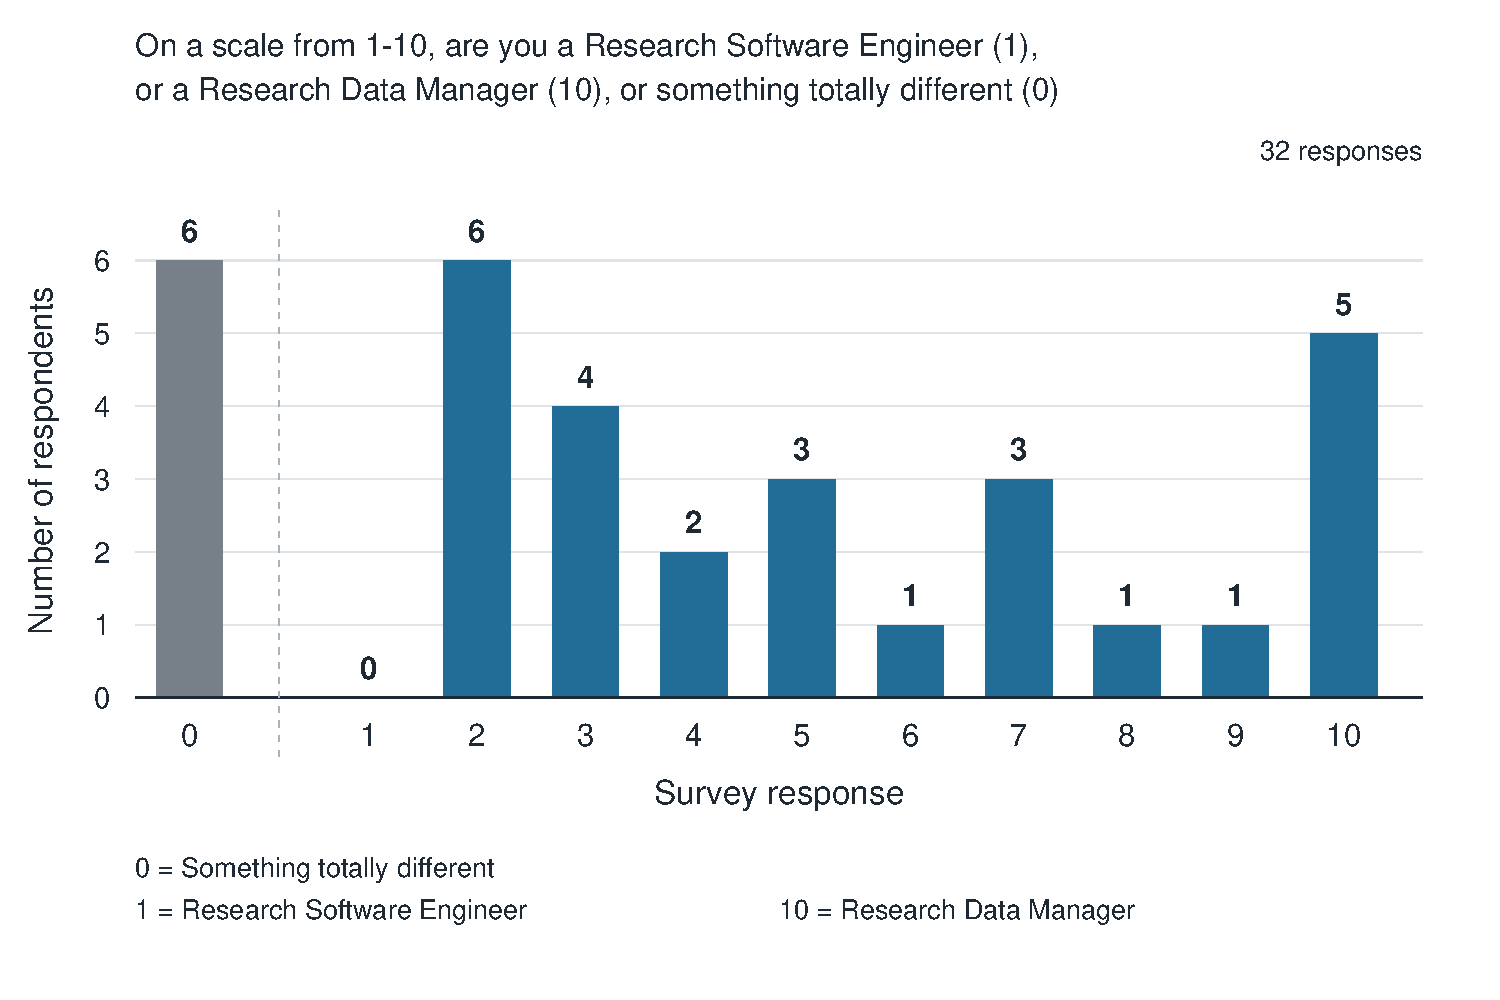
\includegraphics[width=0.98\linewidth]{survey_roles_bar_plot.pdf}
 \caption{ INF project staff see themselves on a spectrum between RSEs (1 on the x-axis) and data
 stewards (10 on the x-axis). We have no data on how people who answered ``Other'' (0 on the x-axis)
 see themselves. }
 \label{fig:figure_plot}
\end{figure}
We also asked about the tools that people are using in their daily work. We see that there is a plethora of tools that are very domain specific.
However, as the word cloud in \autoref{fig:figure_wordcloud} shows, there is a common core of tooling that is shared across INF projects.\\
\begin{figure}[ht]
  \centering
  \includegraphics[width=0.6\linewidth]{fig3.pdf}
  \caption{While there is a broad spectrum of very specialised tools that come from each
 domain, there is also a core of common tooling that is used by everyone.}
 \label{fig:figure_wordcloud}
\end{figure}
We closed the survey with a question about what people would like to see at a follow-up workshop.
Networking, collaboration and the sharing of best practices are, again, very high on the list of requested topics.
\vspace{-1em}\newpage
\section{Lessons Learnt}
\label{sec:lessons}
As we have seen, INF projects have become established across most domains of research.
We observe, that some INF projects lean towards a service-providing idea, where the services
can even be bundled across SFBs such as in \autoref{subsec:vdr}
while others lean towards a project based output.
Irrespective of this, there are still common core questions that each INF project tries to find answers to.
In the in-person workshop, we led discussions in four separate groups.
We summarise each discussion in the following paragraphs.
\vspace{-1em}
\subsection{Outreach, Collaboration and Networking}
INF projects are often one of the cross-cutting components within a CRC,
and therefore they play an important part in the collaboration and networking within the project.
Since partners in INF projects necessarily need a higher-level overview of the work across the entire CRC, 
they can also be valuable partners or even facilitators of project outreach. 
This section discusses experiences in this important social and cross-disciplinary component of an INF project.

We acknowledge that some of the experiences likely only apply to certain categories of domains.
However, we also expect that often these are wide enough, \eg~“the natural sciences”, to be interesting to the reader.
Investigating the breadth of applicability would be valuable to do, however we do not have enough data to make such claims. 
Thus, most of the following has a more anecdotal character. Nevertheless, participants expressed that sharing these experiences 
was valuable for them, and likely also their projects. 

We start with the usual suspects and their perceived effectiveness, rooted in project management.
Most projects hold annual status and PhD candidate meetings.
Both are seen as somewhat useful, but their frequency is perceived as too low.
In contrast, quarterly meetings are experienced as much more effective: 
three months is not too often to interfere with “regular work”, 
but frequent enough to provide early feedback and incentivise timely implementation of agreed-upon targets.
Importantly, this frequency is not only seen as more effective by the INF teams,
but also by the researchers, increasing their engagement with the INF projects.
Relatedly, open development, as opposed to a closed one, eased outreach for multiple INF projects,
as researchers felt more connected to the work within the INF project. 

Another topic besides meeting frequency is the choice of contact channels.
Workshop participants agreed that there is no single preferred channel; rather
the best choice is effectively dictated by the channels the researchers within the CRC already use.
One piece of advice from the workshop is therefore: investigate the preferred communication and outreach channels of your community, and use those. 
While creating networks between non-INF projects was often experienced as easier than between INF and non-INF projects, serving and then re-using their communication channels was often helpful.
Generally, meeting formats with a lower (near-work) level seem to work far better than higher-level formats.
This includes offerings as part of PhD-schools, courses, as well as internal project pairings.
The closer those are to what researchers perceive as “the actual work”, the more successful they are.
One of the prerequisites for success, also more generally,
of these efforts seems to be an explicit backing of such low-level offerings and pairings by the project PIs.
One result is that new topics within digital research, \eg, tools or methods, can sometimes be relatively easy to introduce on a low-level, but may require substantial persuasion on the level of research-PIs.
A key lesson learned is that PI buy-in is not merely beneficial, but a key ingredient for the successful implementation of RDM and RSE practices.

Not surprisingly, general ideas that are close to the Open Science community, and thus to the RDM and RSE communities as well, like the FAIR principles,
can be hard to convey within some CRCs, especially when the served communities do not put a high value on those.
Then, an INF project not only has the role as RDM/RSE-enabling unit, but also as an Open Science evangelist.
\vspace{-2.5em}
\subsection{How do we educate scientists and ourselves?}
Education and training for scientists and research data managers is a multifaceted challenge that goes beyond simply providing access to courses.
We acknowledge that an important task of INF projects is the provision of teaching materials, but the training of the INF project itself is equally important.
While many researchers are capable of identifying and enrolling in online training opportunities independently, a recurring difficulty lies in finding relevant and high-quality training that aligns with their specific needs and contexts.
This highlights the importance of not only curating suitable offerings but also guiding researchers toward them.
A key factor in effective training is the careful tailoring of content to the target audience.
Generic training formats often fall short, particularly when domain-specific tools and practices are involved.
Integrating such specialised tools into training programs remains a significant challenge,
yet it is essential for ensuring applicability in real-world research settings.
Without this alignment, there is a risk of participants losing interest and adopting sub-optimal or ``wrong'' solutions early on. This leads to a kind of ``Good-Enough'' problem,
where initial, partial success obscures underlying issues and may even have long-term negative consequences.

To address these challenges, training efforts should be complemented by consulting services that engage directly with researchers’ specific use cases.
This allows for more targeted support and helps bridge the gap between theoretical knowledge and practical implementation.
In many cases, basic training is already provided by INF teams themselves, but there is clear value in expanding beyond these internal efforts.
Leveraging external training opportunities -- such as those offered externally to the CRC or broader initiatives -- can help diversify and strengthen the available training landscape.
An important dimension is the relationship between different communities, particularly between INF projects and domain researchers.
In some fields, formal certification processes are difficult to establish, partly due to mutual uncertainties and a lack of shared understanding.
This underscores the need for improved communication and information exchange between these communities.
Training is not only relevant for researchers but also for RSEs, Data Stewards, and other support roles, whose professional development is equally important for sustaining high-quality research environments.
In some cases, dedicated positions exist with explicit responsibility for training, extending beyond purely infrastructure-related topics.
However, these roles are often developed “on the job,” and a recurring issue is the lack of recognition through traditional academic outputs such as publications.
Overall, strengthening education and training in this space requires a combination of better curation,
audience-specific design, integration of domain tools, and closer alignment with real research practices.
Equally important are structural improvements, such as fostering cross-community exchange and recognising training-related work as a valuable professional contribution.
\vspace{-1em}
\subsection{Reproducibility, Quality and Validation of created Artefacts}
The workshop discussions established that while automated tools are rapidly advancing, human expertise remains central to artefact validation.
In fields dealing with sensitive clinical or animal data, researchers are increasingly adopting a "human-in-the-loop" approach.
Within this framework, machine learning models and locally-hosted or privacy preserving LLMs are utilised to suggest metadata or classify complex datasets, which are then verified through expert visualisation and manual checks.
This method ensures that data privacy is maintained while leveraging AI to handle the increasing volume of research outputs.
Technical validation becomes more complex as software grows in scale, requiring sophisticated containerisation and environment management.
Participants identified tools such as Pixi and the MaRDI packaging system as essential for managing dependencies and namespaces in large-scale projects.
For dynamic datasets that change over time, static identifiers alone are often insufficient to guarantee reproducibility.
Instead, modular Jupyter notebooks and data chunking strategies are used to document specific states and edge cases, ensuring results can be reconstructed even when the underlying data are not static.
Furthermore, implementing CI/CD pipelines and automated testing allows for the continuous monitoring of software quality, specifically checking for breaking changes or inconsistencies caused by random seeds and stochastic processes.
Finally, the long-term quality of artefacts depends on the rigorous use of ELNs like \href{https://chemotion.net/}{Chemotion}, \elabftw, and Sciformation to capture  experimental procedures and data provenance at the point of origin.
Integrating ELNs with established repositories like \href{https://dataverse.org/}{Dataverse}/\href{https://darus.uni-stuttgart.de/dataverse/darus}{DaRUS} enables structured, metadata-rich publication of experimental data, while version control platforms like GitHub support the parallel management of research software.
Despite these tools, the workshop highlighted a persistent gap in the quality of researcher-provided metadata, pointing to the need for better training and workflow integration to ensure artefacts remain long term verifiable and reusable.
% \vspace{-1em}
\subsection{Workflows and Pipelines}
A common topic occurring in INF projects is helping researchers form pipelines of the software they use.
In this endeavour, especially workflow platforms are particularly beneficial.
Established examples from various domains are \href{https://galaxyproject.github.io/}{Galaxy}, \href{https://esciencelab.org.uk/products/taverna/}{Taverna}, and \href{https://workflowhub.eu/}{workflowhub}.
The use of standardised languages like \href{https://www.commonwl.org/}{CWL} would be beneficial, but so far we see a number of languages
like Mardiflow, \href{https://snakemake.readthedocs.io/en/stable/}{snakemake} and nextflow in use.\\
Another useful mechanism for automated workflows is pipelines,
as offered by platforms such as github and gitlab in their CI/CD environments.
While it would be great to use standardised languages, there are a couple of stumbling blocks that make adoption difficult:\\
Workflow languages require training.
Since you have to lay out your steps in a standardised language, you also have to learn it.
This process is similar to programming, and thus requires coding practice.
Codified pipelines will have version changes, and that can bring the well-known problem of long-term maintenance.
For some, an issue can be that workflows have to be permitted in the respective domain,
so it can be that the use of a workflow requires approvals, \eg~by an ethics board or similar.
While certainly appealing to INF projects, the participants noted that
workflow languages currently definitely have a low reach into the user base.\\
Other topics that hinder adoption are the availability of the inputs to the workflows.
Findability of the respective responsible users can be a problem, or
it can be difficult to get the permission to use input data.
% Re-Use and Maintenence are an issue.
Limited awareness of automation benefits often prevents people from getting started.
Possible solutions that the participants discussed are the use of an RAG (Retrieval-Augmented Generation) supported Chat-Agent for scientists,
or easy/good documentation.
\vspace{-1em}
\section{Summary}
Comparing the initial problems of the INF projects in \autoref{sec:history}
with the actual tasks that INF projects perform in \autoref{sec:inf-in-germany}
and what we identified as ongoing challenges in the workshop in \autoref{sec:lessons}
we observe that technical challenges have evolved, while the human factor still is tricky ---  noting that no one reported on
the failure of an INF project \cite{Dierkes2020}.
We observe that the provision of long-term storage does not pose such a large issue anymore.
This has often either been solved within the CRC or through collaborations with institutions within the universities or within the framework of the NFDI.
This points to a greater shift in the landscape surrounding the INF projects.
Libraries and compute centres themselves offer to become part of the CRC proposals as evidenced by examples from \autoref{subsec:vdr}, the literature \cite{Hausen_Rosenberg_Trautwein-Bruns_Schwarz_2020},
and generalised into a template form in \cite{Kempf2026}.\\
Getting support as an INF project is an ongoing challenge that is helped by numerous networks.
The formation of the NFDI in 2020 brought a new push to the available networks for the INF projects, since
the consortia now form a domain specific network of sorts.
Also, numerous RDM specific networks emerged, like \href{https://saxfdm.de/}{SaxFDM}, that offer local, RDM specific networks.
INF projects leaning into software development have found networks in the \href{https://de-rse.org/}{RSE} movement.\\
Also in this manuscript, we have categorised INF projects where they lie on the RSE-RDM spectrum, but more broadly speaking,
these are all instances of \href{https://drtp-skills.ac.uk/}{dRTPs}, digital Research Technical Professionals.
INF projects will probably be even more diverse, if data scientists, AI specialists and other dRTPs can provide skills useful for the CRCs.
At the same time, INF projects increasingly fulfil an important mediating role between domain scientists, 
institutional infrastructure providers, and national initiatives such as the NFDI. Beyond providing technical solutions, 
they translate evolving requirements between communities with different practices, expectations, and technical backgrounds. 
This bridging function is becoming ever more critical as collaborative and data intensive research continues to grow in complexity.
So with respect to the communities and the professionalisation the INF projects have matured, but what has stayed the same?
INF projects in CRCs are subject to the project based funding of the DFG, therefore the CRC itself cannot provide a stable position.
This also brings up again the unresolved problem of how to provide continuity across personnel rotations in INF projects.
It is encouraging to see that libraries and compute centres are stepping up here, since these are institutions that
can provide long-term career perspectives for experts employed in INF projects and can provide a fallback in the case of rotations.
Hopefully, in the future more improvements can be made \eg, by combining the political voice of the data stewards and the RSE movement.\\
Comparing with \cite{mueckschel2006} a couple of other challenges still persist, such as INF projects struggling
to adapt their platforms to the scientists’ evolving requirements, or how to design platforms that are open and extensible
while still being easy enough to be accepted by users.
We have detailed some of these struggles and some of this generation’s solutions in our lessons learnt in \autoref{sec:lessons}.
Adapting to rapidly changing scientific questions will always be a challenge to the people filling out the role of the INF project in a CRC.
But together with the strong networks they are embedded in\footnote{
We founded a network for INF projects: \url{https://www.listserv.dfn.de/sympa/info/inf-projects-in-crcs}.
}, this is a challenge that INF projects everywhere happily take on.


\begin{acknowledge}
We thank the university of Stuttgart for the hospitality to host this workshop.
AA acknowledges funding from the DFG, TRR 265 "Losing and Regaining Control over Drug Intake: From Trajectories to Mechanisms to Interventions", project  Z/INF - project number \geprislink{402170461}.
AG, SJ, RM, PR, and HR acknowledge funding from the DFG, TRR 391 "Spatio-temporal Statistics for the Transition of Energy and Transport'' (\geprislink{520388526}).
FG acknowledges funding from the DFG, CRC 1170 “Tocotronics”, project Z03 - project number \geprislink{258499086}.
FL acknowledges funding from the Klaus Tschira Foundation through project “FutuRSI” (00.048.2024).
HO acknowledges funding from the DFG, CRC 1313 “Interface-Driven Multi-Field Processes in Porous Media – Flow, Transport and Deformation”, project INF - project number \geprislink{327154368}.
JF acknowledges funding from the DFG, TRR~408 /1 2025 – project number: \geprislink{531327426}, project INF.
JSG and MH acknowledge funding from the DFG through the TRR 379 "Neuropsychobiology of Aggression", project INF - project number \geprislink{512007073}, and the CRC 1451 "Key Mechanisms of Motor Control in Health and Disease", project INF - project number \geprislink{458705875}.
LS acknowledges funding from the DFG, TRR 393 "Trajectories of Affective Disorders: Cognitive-Emotional Mechanisms of Symptom Change", project  Z/INF - project number \geprislink{521379614}.
MG, MP, LFB, AM, FP acknowledge funding from the DFG, TRR 418 ``Foundations of Circadian Medicine'', project INF - project number \geprislink{541063275}.
MJ, TP, FP acknowledge funding from the DFG, CRC 1340 "Matrix in Vision", project INF - project number \geprislink{372486779}.
MM acknowledges funding from DFG, CRC 1646/1 2024 -- \geprislink{512393437}, project INF.
MMB acknowledges funding from DFG, CRC 1629 ``Negation in Language and Beyond'', project INF - project number \geprislink{537324246}.
MMB acknowledges the contributions of the INF members in CRC 1629: Sol Lago, Alexander Mehler, Manfred Sailer, Giuseppe Abrami, Nasimeh Bahmanian, Leon Hammerla, and Andy Lücking.
ND acknowledges funding from DFG, CRC 1638, project INF - project number \geprislink{511488495}.
RD thanks the DFG for its support through the CRC 1415 "Chemistry of Synthetic Two-Dimensional Materials", project INF - project number \geprislink{417590517}.
VD acknowledges funding from the DFG Project-ID \geprislink{388390466}-TRR 247 (subproject INF) and CRC~1625, project number \geprislink{506711657} (subproject INF).
DY, MA, FJ, and KY acknowledge funding from the DFG, TRR 410 "WETSCAPES2.0: Sinks, Links and Legacies of Novel Ecosystems in Rewetted Fen Landscapes", project Z03 -- project number \geprislink{531801029}.
\end{acknowledge}

\begin{aiuse}
AI has been used for copy-editing purposes.
\end{aiuse}

\begin{data}
For data privacy reasons, we only list aggregated data in this publication.
\end{data}

\bibliographystyle{eceasst}
\bibliography{report}

\end{document}
